%%%--- Template for master thesis at SfS
%%%--- Modified template with more comments and examples -- SG, 11/06/09
%%%------
\documentclass[11pt,a4paper,twoside,openright]{report}
%%not needed \usepackage{E}
\usepackage[utf8]{inputenc}
\usepackage[english]{style/ETHDAsfs}%--> ETHDASA + fancyheadings + ... "umlaute"
%  + sfs-hyper -> hyperref

\usepackage{pdfpages}%%to include the confirmation of originality (plagiarism
\usepackage{amsbsy}%% for \boldsymbol and \pmb{.}
\usepackage{amssymb}%% calls  amsfonts...
\usepackage{booktabs} % For \toprule etc. in tables
\usepackage[table]{xcolor} 
%or \usepackage{german8}%-- =  german  +  isolatin1
\usepackage{graphicx}%-- f?r PostScript-Grafiken (besser als  psfig!)
%\usepackage[draft]{graphicx} % grafics shown as boxes --> faster compilation
%
\usepackage[longnamesfirst]{natbib}%was {sfsbib}%- F?r  Literatur-Referenzen
%           ^^^^^^^^^^^^^^ 1) "Hampel, Ronchetti, ..,"  2) "Hampel et al"
% Engineers (and other funny people) want to see [1], [2]
% ---> use 'numbers' : \usepackage[longnamesfirst,number]{natbib}
%
%
\usepackage{style/texab}%- 'tex Abk?rzungen' /u/sfs/tex/tex/latex/texab.sty
        %%- z.B.  \R, \Z, \Q, \Nat f?r reelle, ganze, rationale, nat?rl. Zahlen;
        %%-       \N   (Normalvert.)  \W == Wahrscheinlichkeit .....
        %%-  \med, \var, \Cov, \....
        %%-  \abs{x} == |x|   und   \norm{y} ==  || y ||   (aber anst?ndig)
%% NOTE: texab contains many useful definitions and "shortcuts". It is
%% worth to open the file and have a look at them. HOWEVER, some
%% definitions can lead to conflicts with other packages. You
%% might for example want to comment out the line defininf \IF as an
%% operator when working with the algorithmic package, or to comment out
%% the line defining a command \Cite with working with the Biblatex package
\usepackage{amsmath}
%\usepackage{mathrsfs}% Raph Smith's Formal Script font --> provides \mathscr
\usepackage{enumerate}% Fuer selbstdefinierte Nummerierungen
\usepackage{longtable}
\usepackage[font={small,sl},labelfont={bf},format=hang,indention=-0.5cm,labelsep=endash]{caption}
\usepackage{rotating}
%--------
\usepackage{relsize}%-> \smaller (etc) used here
\usepackage{color} %% to allow cloring in code listings
\usepackage{listings}% Fuer R-code, C-code, ....  and settings for these:
\definecolor{Mygrey}{gray}{0.75}% for linenumbers only!
\definecolor{Cgrey}{gray}{0.4}% for comments
\lstloadlanguages{R}
\lstset{ %% Hilfe unter z.B. http://en.wikibooks.org/wiki/LaTeX/Packages/Listings
language=R,
basicstyle=\ttfamily\scriptsize,%%- \small > \footnotesize > \scriptsize > \tiny
%commentstyle=\ttfamily\color{Cgrey},
commentstyle=\itshape\color{Cgrey},
numbers=left,
numberstyle=\ttfamily\color{Mygrey}\tiny,
stepnumber=1,
numbersep=5pt,
backgroundcolor=\color{white},
showspaces=false,
showstringspaces=false,
showtabs=false,
frame=single,
tabsize=2,
captionpos=b,
breaklines=true,
%breakatwhitespace=false,
keywordstyle={},
morekeywords={},
xleftmargin=4ex,
literate={<-}{{$\leftarrow$}}1 {~}{{$\sim$}}1}
\lstset{escapeinside={(*}{*)}} % for (*\ref{ }*) inside lstlistings (Scode)
%%----------------------------------------------------------------------------

%%------- Theoreme ---
\newtheorem{definition}{Definition}[subsection]
\newtheorem{lemma}[definition]{Lemma}
\newtheorem{theorem}[definition]{Theorem}
\newtheorem{Coro}[definition]{Corollary}
\theoremstyle{definition}
\newtheorem{example}[definition]{Example}
\newtheorem*{note}{Note}
\newtheorem*{remark}{Remark}

\DeclareMathOperator*{\plim}{plim}
% \def\MR#1{\href{http://www.ams.org/mathscinet-getitem?mr=#1}{MR#1}}

% \newcommand{\Lecture}[3]{\marginpar{#3.#2.#1}}
% \newcommand{\Fu}{\mathcal{F}}
\newcommand{\aatop}[2]{\genfrac{}{}{0pt}{}{#1}{#2}}

%\renewcommand{\theequation}{\arabic{equation}}
%\numberwithin{equation}{subsection}

%%%%%%%%%%%%%%%%%%%%%%%%%%%%%%%%%%%%%%%%%%%%%%%%%
%%% Path for your figures                      %%%
%%%%%%%%%%%%%%%%%%%%%%%%%%%%%%%%%%%%%%%%%%%%%%%%%
% Set the paths where all figures are taken from:
\graphicspath{{images/}}

%%%%%%%%%%%%%%%%%%%%%%%%%%%%%%%%%%%%%%%%%%%%%%%%%
%%% Define your own commands here             %%%
%%%%%%%%%%%%%%%%%%%%%%%%%%%%%%%%%%%%%%%%%%%%%%%%%
\newcommand{\Bruch}[2]{{}^{#1}\!\!/\!_{#2}}
\renewcommand{\labelenumi}{\roman{enumi}.)}
\providecommand{\tightlist}{%
  \setlength{\itemsep}{0pt}\setlength{\parskip}{0pt}}

\makeatletter
\@ifundefined{Shaded}{
}{\renewenvironment{Shaded}{\begin{kframe}}{\end{kframe}}}
\makeatother


\begin{document}
\bibliographystyle{apalike}%style/chicago}% ---> Hampel,F., E.Ronchetti,... W.Stahel(1986) ...
 %was \bibliographystyle{sfsbib}\citationstyle{dcu} %OR DEFAULT : \citationstyle{agsm}

\pagenumbering{roman}%- roman numbering for first few pages

%%%%%%%%%%%%%%%%%%%%%%%%%%%%%%%%%%%%%%%%%%%%%%%%%
%%% Title page                                %%%
%%%%%%%%%%%%%%%%%%%%%%%%%%%%%%%%%%%%%%%%%%%%%%%%%
\period{September 2024}
\dasatype{Master Thesis}
\students{Marco Froelich (22-942-601)}
\alternatereaderprefix{Co-Adviser:}
\alternatereader{Dr.~Matthias Rothlisberger}
\mainreaderprefix{Adviser:}
\mainreader{Prof.~Dr.~Nicolai Meinshausen}


\submissiondate{September 16th, 2024}
\title{Investigating year-to-year variability of hot extremes and contributions from heat-generating mechanisms}

\maketitle%- Titelseite wird abgeschlossen
\cleardoublepage
 %%~~~~~~~~~~~~~~~~~~~~~~~~~~~~~~~~~~~~~~~~

%%%%%%%%%%%%%%%%%%%%%%%%%%%%%%%%%%%%%%%%%%%%%%%%%
%%% Insert here acknowledgements and abstract %%%
%%%%%%%%%%%%%%%%%%%%%%%%%%%%%%%%%%%%%%%%%%%%%%%%%
%% Dedication (optional)
%\markright{}
%\vspace*{\stretch{1}}
%\begin{center}
%    To some special person
%\end{center}
%\vspace*{\stretch{2}}

% Preface (optional)
\newpage
\markboth{Preface}{Preface}
\chapter*{Preface}

I would like to extend my gratitude to all the people that supported me throughout the this project. To Matthias, that from the start of my interest in this field, inspired and challenged me to create something new. You taught me many lessons that will stay with me and I value enormously the interesting conversations that stimulated a lot of excitment and creativity. To Maybritt, thank you for your support, insights, supervision and the many conversations that inspired solutions. Your encouragements from the start to the end were incredibily valuable. To Belinda, your help was essential in fortifying my physics competences and I appreciated the time you spend supporting my work. To Heini, thank you for the supervision and feedback that was instrumental in shaping a meaningul and impactful project. You all showed interest in my work and I am very grateful to have had such a competent, enthusiastic and friendly team.

This thesis has been a unique opportunity to place myself at the head of a scientific project, and it was foremost a humbling experience, as the challenges of interdisplinary research have taught me. Throughout all the ups and down, I would like to thank my friends for the moments of laughter, for being great rubber ducks, and for all the good times. I will miss you all a lot and am eager to follow all your future adventures. Grazie mamma per essere stata sempre raggiungibile, per le poesie ispirante e le foto del grigio che mi fanno sorridere molto. Merci papa pour ces parties de ping-pong qui me sont si importantes et les bons verres de vins. To Matt and Luca, always wonderful to have you around: I cherish all the moments we have together. To my Manu, thank you for everything. Your calls and visits brought me joy and comfort, our time together is so dear to me and you are always an inspiration. I am so glad to have you by my side. 


%%% Local Variables: 
%%% mode: latex
%%% TeX-master: "MasterThesisSfS"
%%% End: 


% Abstract should not be longer than one page.
\newpage
\markboth{Abstract}{Abstract}
\chapter*{Abstract}

Heat-related extremes are important meteorological phenomena that can have strong consequences on human health and the environment. Climate change is expected to exacerbate these impacts through an increase in the frequency of hot extreme occurrence and intensity. Although there exists abundant literature on the typical physical functioning of these events and their association to the variability of the climate system on different temporal scales, there lacks a global assessment of the influence of major physical processes - heat advection, adiabatic compression and diabatic heating - on the yearly variation of hot extreme magnitudes. To remediate this knowledge gap, we first propose a data-driven, systematic analysis of second-moment characteristics of yearly maxima near-surface hot extreme events and contributing heat-generating processes. Second, we apply deep-learning methods to model hot extreme Lagrangian trajectories to gain insights into important dynamical features. No physical process is globally found to dominate variability in these events and significant variance contributions exist from at least two processes, suggesting that mean-state understanding of hot extreme development may not not be sufficient to explain large year-to-year differences in their magnitudes. Furthermore, this analysis reaffirms the presence of strong dependencies between the three physical mechanisms leading to a characterization of their variability by only one or two degrees of freedom in most of the world. Finally, the approach for the analysis of parcel trajectories was limited due to generally poor predictive performance, but showed that the patterns in advective, adiabatic and diabatic temperature anomaly generation follow patterns that may be predicted from their history, encouraging for future work. In addition, over oceans and many land regions we observe that adiabatic heating is minimal during the final 24h, suggesting that hot extreme primarily descend to the surface earlier than a day before, thus leading to contributions from advective and diabatic processes more likely.

%%% Local Variables: 
%%% mode: latex
%%% TeX-master: "MasterThesisSfS"
%%% End: 



%%%%%%%%%%%%%%%%%%%%%%%%%%%%%%%%%%%%%%%%%%%%%%%%%
%%% Table of contents and list of figures and %%%
%%% tables (no need to change this usually)   %%%
%%%%%%%%%%%%%%%%%%%%%%%%%%%%%%%%%%%%%%%%%%%%%%%%%
\newpage
\tableofcontents
%\newpage
%\listoffigures
%\newpage
%\listoftables

%% Notations and glossary (optional)
%\cleardoublepage
%\phantomsection
%\addcontentsline{toc}{chapter}{\protect\numberline{}{Notation}}
%\markboth{Notation}{Notation}
%\chapter*{Notation}
\label{c:Notation}

Explain your symbols and abbreviations.

%%% Local Variables: 
%%% mode: latex
%%% TeX-master: "MasterThesisSfS"
%%% End: 


\cleardoublepage
\pagenumbering{arabic}%--- switch back to standard numbering


%%%%%%%%%%%%%%%%%%%%%%%%%%%%%%%%%%%%%%%%%%%%%%%%%
%%% Your text... Either write here directly,  %%%
%%% or even better: write in separate files   %%%
%%% that you just have to include here.       %%%
%%%%%%%%%%%%%%%%%%%%%%%%%%%%%%%%%%%%%%%%%%%%%%%%%
\chapter{Introduction}\label{introduction}

\section{Motivation}\label{motivation}

In recent years, heat-related near-surface extreme events have globally become increasingly important. These include hot extremes and heatwaves, that we characterized by short, sudden spikes in temperatures and periods of prolonged positive temperature anomalies, respectively. Hot extremes in particularly impact human health through high mortality and morbidity rates in certain demographics \citep{medina-ramon_temperature_2007,oudin_astrom_heat_2011,green_impact_2019,ebi_hot_2021}; can be damaging to agricultural and ecological systems through productivity decreases and heat stress \citep{teixeira_global_2013,gourdji_global_2013,vogel_effects_2019}; and may pressure national economies by increasing energy demands \citep{perera_quantifying_2020} compounded with damage to thermal-power plant infrastructure \citep{entriken_impacts_2012}, as well as lowering labor productivity \citep{garcia-leon_current_2021}. Furthermore, climate change is expected to exacerbate hot extreme impacts through an increase in the frequency of their occurrence and their intensity \citep{slater_substantial_2021,fischer_increasing_2021,thompson_2021_2022}. Uncovering the associations between hot extreme event magnitudes and the processes associated with the development of such events is therefore crucial for more robust understanding of future changes in extremes, leading to potential improvements in forecasting capabilities for emergency warning systems and supporting future adaptation and mitigation strategies.

Coupled with increasing mean global temperatures, recent record-shattering events highlight the importance of understanding not only the evolution and drivers of typical hot extremes, but also their variability. The Pacific North-West 2021 event is particularly illustrative, breaking the national temperature record by more than 4°C and leading to more than a thousand deaths \citep{white_unprecedented_2023}. \cite{lin_2021_2022} demonstrated that no ensemble member resolved such intense temperature 10 days before the event while analysis by \cite{lucarini_typicality_2023} suggested this event may become typical when conditioning on the existence of large and persistent temperature anomalies locally. Uncovering the physical differences that separate such rare events from lower-intensity hot extremes will provide insights into improving forecasting, in addition to furthering understanding of how they may evolve under climate change.

Although a good general understanding of mean-state hot extreme evolution exists and more detailed assessments have been made regionally to compare specific high-impact events, a knowledge-gap exists in quantifying the contribution of known physical processes to hot extreme magnitude variability globally. This thesis attempts to close this gap by first proposing a systematic analysis of second-moment characteristics of hot extreme events and second applying state-of-the-art deep-learning methods to uncover patterns in trajectory features important for the development of hot extremes.

\section{Outline}\label{outline}

A comprehensive overview of hot extreme literature and a review of important meteorological background is presented in \hyperref[meteorological-background]{Chapter 2}. In addition, it will introduce the work that this thesis is based upon and extends. \hyperref[data]{Chapter 3} will describe the data used and illustrate some representative examples. \hyperref[statistical-methods]{Chapter 4} will motivate and explain the employed methodologies, as well as provide the statistical background required to understand them. \hyperref[results]{Chapter 5} will present and discuss the obtained results. \hyperref[conclusion]{Chapter 6} offers a broader discussion on the findings of this thesis, summarizes the work and suggests avenues for future research.

\chapter{Meteorological Background}\label{meteorological-background}

It is important to recognize that the literature on heat extremes presents diverse and at times contradictory definitions of hot events. In this report, a `hot extreme event' will describe an anomalously high spike in near-surface temperature occurring over the timescale of a day. A `heatwave' will then describe an event of prolonged anomalously high near-surface temperature on the order of multiple days or weeks. In addition to reviewing literature on hot extremes, this section discusses heatwave research as they, although being distinct, often evolve together \citep{robinson_definition_2001}.

\section{Mechanisms of hot extreme development}\label{mechanisms-of-hot-extreme-development}

The temperature of a volume of air - generally referred to as an air parcel in atmospheric sciences - can increase due to three primary mechanisms: warm \textbf{advection} involves the horizontal transport of warmer air parcels into a climatologically colder region; \textbf{adiabatic heating} is the result of descending air that compresses and thus heats; \textbf{diabatic heating} involves radiative effects including sensible heat fluxes from the Earth's surface. These mechanisms provide a foundation to discuss atmospheric phenomena linked to hot extreme evolution and suggest a methodology, later discussed, to quantify the contribution of each physical processes to specific events.

In the mid-latitudes, anticyclonic flow situations serve as the basis for hot extreme development \citep[e.g.][]{pfahl_quantifying_2012}. They are often associated with atmospheric blocks - a pattern characterized by persistent anticyclonic activity that prevents the influence of the prevailing flows \citep{lupo_atmospheric_2021} - or amplified and quasi-stationary ridges \citep{sousa_european_2018}. Thereby, they develop regions of large subsidence and clear skies conducive to strong radiative heating in summer \citep{lupo_atmospheric_2021}. Indeed, atmospheric blocks co-locates with hot extremes, particularly well over the Northern \citep{pfahl_quantifying_2012,bieli_lagrangian_2015,brunner_dependence_2018} and Southern \citep{pezza_severe_2012} mid-latitudes, although with significant spatial variability and large land-ocean contrasts. Over Europe, increased sensible heat fluxes from decreased soil moisture content and/or hydrological pre-conditioning are partly responsible for the observed land patterns, while the land-ocean contrast may be explained by a lower temperature variability due to water's larger heat capacity.

In the polar latitudes, a diversity of atypical mechanisms may evolve due to the presence of snow and ice-sheets. Generally, an enhanced albedo effect implies lower diabatic heating and the temperature inversion created by a cold surface temperature limits adiabatic heating. Furthermore, ice-sheets are found at relatively high altitudes \citep{fretwell_bedmap2_2013} leading to adiabatic cooling from air parcels that ascend from coastal regions. Some studies have also suggested that intrusions of sub-polar air into the Arctic, such as by atmospheric rivers (AR) - corridors of rapidly ascending sub-tropical air that transport moisture and heat towards the poles - may disturb the polar climate \citep{ma_wintertime_2024, papritz_role_2023}. This may lead to increasing downward longwave radiation that accelerates sea-ice melting \citep{kapsch_springtime_2013, mortin_melt_2016} and advective warming at both lower and upper levels \citep{papritz_role_2023}. Indeed, a case-study on the March 2022 East Antarctica heat extreme showed that intense atmospheric blocking initiated by an AR led to the weakening of the ice-sheet temperature inversion, intensifying adiabatic heating from subsiding air \citep{wille_extraordinary_2024}.

In the tropics, the weather is predominantly influenced by circulation anomalies (such as the El-Nino Southern Oscillation - ENSO) and local moist convective systems (although anti-cyclonic activity may still be a major synoptic driver). The limited literature on tropical hot extremes and heatwaves has found a strong association of hot extreme events with dry land conditions, indicative of strong coupling between land-surface processes and the atmosphere: anti-cyclonic activity yielding clear skies may enhance radiative heating and reduce soil-moisture \citep{geirinhas_climatic_2018,costa_most_2022}, in turn decreasing the potential of latent cooling - the loss of heat due to evaporation - and increasing sensible heat fluxes. Theoretical work by \cite{byrne_amplified_2021} suggested that the onset of moist convection increases relative humidity which limits the growth of positive temperature anomalies.

Soil moisture and its complex dependence with near-surface temperature is not only important in the tropics, but also in the extra-tropics. Low soil-moisture content - dried by warm advection - is associated with increased sensible heating and decreased latent heating, which can reduce the potential for precipitation from deep convection and/or support a blocking high-pressure system, thus enhancing dry conditions \citep{berg_impact_2014,wang_sensitivity_2019,miralles_mega-heatwave_2014,schumacher_amplification_2019}. \cite{wehrli_identifying_2019} showed that contributions from thermodynamic drivers such as soil moisture deficits are as important as circulation divers in 5 recent heat wave events. In the context of climate change, \cite{vogel_effects_2019} quantified the contribution of these soil moisture and temperature feedbacks to regional increase in TX1day magnitude at more than 70\% in Central Europe and Central North America, and around 50\% in Amazonia, Northern Australia and Southern Africa. These mechanisms may evolve differently on small or relatively large temporal and spatial scales \citep{mccoll_short-term_2019}, further illustrating their complexity. However, a systematic and global analysis of their contribution to yearly hot extremes still lacks.

Hot extreme events over oceans have received little attention in the literature, likely due to their smaller impact on society. The absence of land-surface processes in the extra-tropics is expected to lead to a stronger influence of the large scale dynamics on hot extreme development, with adiabatic heating in the subsidence regions of the Hadley cell and advective warming in the mid-latitudes. Furthermore, we expect that regions with cooler sea surface temperatures (SSTs) than air temperature experience diabatic cooling, while in the tropics and over warm poleward currents, the opposite situation might be important with a warmer ocean surface inducing positive diabatic contributions. These processes may also involve coupling with marine heatwave, although this goes beyond the scope of this research.

\section{Global quantification of physical mechansisms}\label{global-quantification-of-physical-mechansisms}

\cite{rothlisberger_quantifying_2023} was the first study to present a global quantification of the contribution of physical processes to hot extreme events. By considering the history of atmospheric air responsible for hot extreme events, it proposes a decomposition of the final temperature anomaly into the temperature anomaly gained through advective, adiabatic and diabatic processes. The methodology and the dataset created forms the basis of this thesis, and an in-depth description is presented in \hyperref[temperature-anomaly-decomposition]{Chapter 4.1}.

The analysis then quantifies the average influence of each process on hot extreme temperature anomaly magnitude (\ref{fig:decompmean}). It showed that hot extreme events in higher latitudes and over land tend to have larger temperature anomalies than over the tropics and over oceans. The regions with largest temperature anomalies are in northern Russia and southern Australia. In addition, no single physical process is found to be dominant in the generation of temperature anomaly, leading to diverse geographical patterns for all three physical processes. The findings mostly agrees with the aforementioned literature, with exceptions over mountainous regions and isolated continental regions.

\begin{figure}
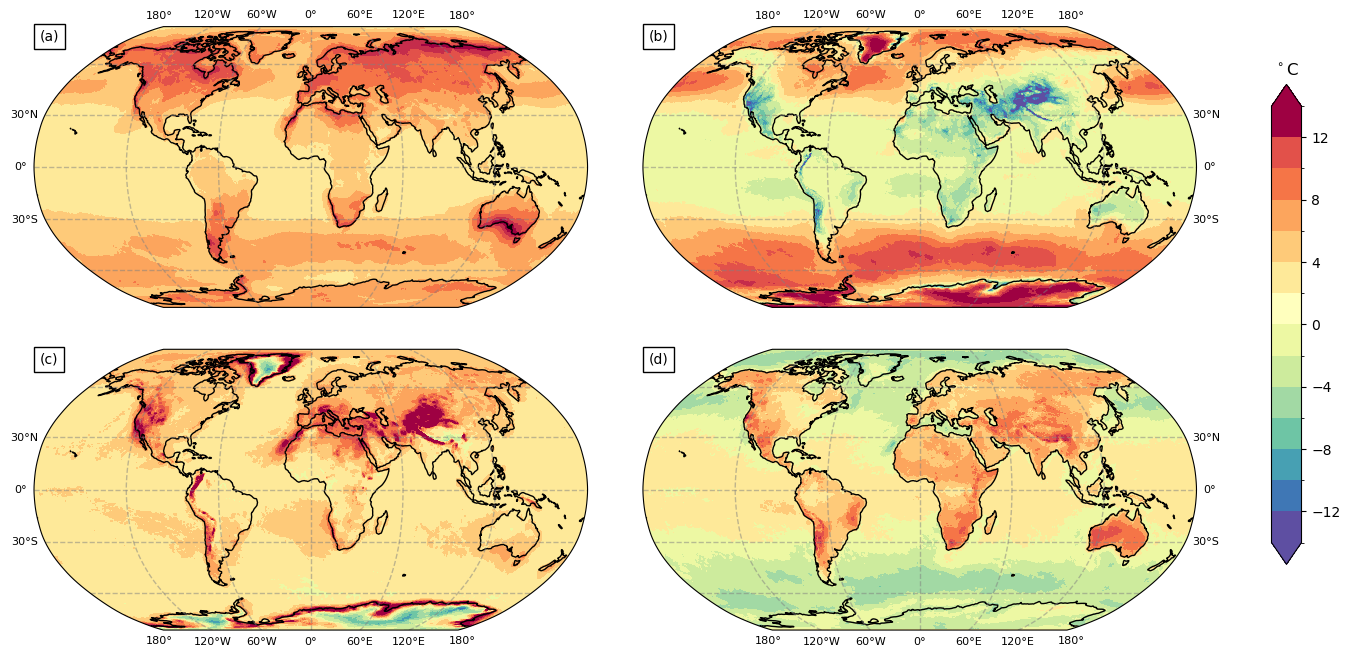
\includegraphics[width=1\linewidth]{images/mean_contribution} \caption{Reproduced from \cite{rothlisberger_quantifying_2023}. The maps plot at every location the mean magnitude of (a) the temperature anomaly and the anomaly contribution from (b) advective, (c) adiabatic and (d) diabatic processes for yearly maxima TX1day events from 1980 to 2020.}\label{fig:decompmean}
\end{figure}

\section{Variability of hot extreme events}\label{variability-of-hot-extreme-events}

So far, we have focused on the understanding of diverse mechanisms that yield hot extreme events across the globe. Several studies have however focused on relating the temporal variability of these processes to the resulting hot extremes variability. Here, variability is a measure of spread observed in a quantity across a temporal scale (daily, seasonally, yearly, etc.). In the European mid-latitudes, changes in variability have been attributed to an increase in anticyclonic activity and advective heating \citep{lenderink_summertime_2007,horton_contribution_2015,holmes_robust_2015} and to the local effects of soil-moisture \citep{quesada_asymmetric_2012,whan_impact_2015,donat_regional_2017,vogel_effects_2019}. \cite{wang_decadal_2023} drew similar conclusions for Asian mid-latitudes, further relating anti-cyclonic activity increases to the North Atlantic Oscillation.

The distribution of regional-to-global hot extremes is expected to both shift positively in the mean and undergo changes in variability due to climate change \citep{lewis_evolution_2017,mckinnon_changing_2016,slater_substantial_2021,fischer_increasing_2021,thompson_2021_2022}. \cite{simolo_quantifying_2022} indeed suggested that daily temperature variability changes are more important than the observed warming trend in explaining amplifications in a majority of identified hotspot regions. In an attempt to relate these changes to dynamics, \cite{fischer_future_2009} quantified the projected changes in hot extreme variability over Europe with respect to the processes associated with inter-annual, intra-seasonal and summer seasonal variability, finding the largest contribution from the former. \cite{di_luca_contribution_2020} quantified the contributions of annual and diurnal first and second-moment features to daily hot extremes over land, showing a diversity of global patterns. \cite{suarez-gutierrez_dynamical_2020} suggested instead investigating variability changes with regard to dynamical and thermodynamical sources in European mid-latitudes, and concludes that the former - encompassing effects of atmospheric blocking - is the main driver of hot extreme variability. However, these approaches lack a direct interpretation since the temporal features may be associated with different physical processes in different regions.

\section{Methods in hot extreme literature}\label{methods-in-hot-extreme-literature}

The weather extremes literature uses two main methodologies: sensitivity and trajectory analysis. To motivate the following work, we give a brief overview of these approaches:

\textbf{Sensitivity analysis} (SA) is the most widely adopted approach to study the effects of initial conditions and model parameters on outputs of a system. It involves running different experiments with simulation tools (including numerical and data-driven models) and assessing the changes in distribution of the response. Formally, sensitivity is defined as the partial derivative of the response with regard to a predictor of interest. It is then related to causality: if one assumes a linear structural model, sensitivity is a measure of the causal effect of a variable on the response. SA literature has considered both local and global measures of sensitivity. The former involves evaluating the sensitivity at a given predictor value and therefore cannot conclude general causal relationships without strong assumptions. The latter presents a difficult problem and different approaches have been proposed that include many typical statistical estimators \citep{razavi_what_2015}.

\textbf{Trajectory analysis} (TA) follows the changes to air parcels along their flow within a dynamical system. This approach takes a Lagrangian perspective, as opposed to the Eulerian perspective that trackes changes to a volume of air at a fixed spatial coordinate. In the context of extreme weather, TA often involves the identification of an event within a numerical model followed by calculation of the flow backwards in time. The output is a timeseries of physical and model quantities that describe the state history of the parcel which gave rise to the extreme event. These characteristics have been used both to understand single events in case-studies \citep[e.g.][]{stohl_lagrangian_2004,huang_moisture_2015,papritz_novel_2023} as well as to gain a general understanding of drivers of extreme weather by aggregation of multiple events \citep[e.g.][]{bieli_lagrangian_2015,quinting_southeastern_2017,rothlisberger_quantifying_2023}.

This thesis uses TA to focus on process understanding of hot extreme development and will expand existing literature, introduced below.

\section{Temperature anomaly decomposition}\label{temperature-anomaly-decomposition}

This investigation is based on a Lagrangian decomposition of temperature anomaly \citep{rothlisberger_quantifying_2023}, which quantifies the contributions of advective (adv), adiabatic (adiab) and diabatic (diab) processes in the generation of temperature anomaly (\(T'\)). Based on \(T'\) - i.e.~temperature anomalies instead of absolute temperature - it leads to a more natural interpretation of the contributors, since some processes of interest - such as warming from horizontal advection - arize due to the presence of anomalously warm air within a dynamic environment.

At location \(\mathbf{x}\) and starting time of the backward trajectory \(t_0\), \(T'\) may be decomposed as follows:

\begin{equation}
\begin{alignedat}{2}
   T'(\mathbf{x},t_X) = & - \int_{t_g}^{t_0} \frac{\partial \bar{T}}{\partial t} \, \text{d}\tau && \qquad \text{seas} \\
   & - \int_{t_g}^{t_0} \boldsymbol{\nu} \boldsymbol{\nabla}_h \bar{T} \, \text{d}\tau && \qquad \text{adv} \\
   & + \int_{t_g}^{t_0} \left[ \frac{\kappa T}{p} - \frac{\partial +  \bar{T}}{\partial p}\right] \omega \, \text{d}\tau && \qquad \text{adiab} \\
   & + \int_{t_g}^{t_0} \left( \frac{p}{p_0} \right)^\kappa \frac{\text{D}\theta}{\text{D}t} \, \text{d}\tau && \qquad \text{diab}
\end{alignedat}
\label{eq:tdecomp}
\end{equation}

where \(\bar{T}\) the temperature climatology; \(t_g < t_X\) genesis time, the time at which \(T'\) was last zero; \(\boldsymbol{\nu}\) the horizontal wind velocity; \(\boldsymbol{\nabla}_h\) the horizontal temperature gradient; \(p\) pressure; \(\omega\) vertical velocity; \(\theta\) potential temperature.

To study hot extremes globally and systematically, \cite{rothlisberger_quantifying_2023} applied \eqref{eq:tdecomp} to yearly maxima of 1-day temperature anomaly averages - denoted TX1day - at every grid point in ERA5 (further described in \hyperref[data]{Data}). Timeseries of backward trajectories - calculated with LAGRANTO \citep{sprenger_lagranto_2015} - are numerically integrated to approximate the integrals. Since weather phenomenon might result from different flows, for yearly maxima event at each grid-point a total of 24 backward trajectories - corresponding to near-surface trajectory starts at 10, 30, 50 hPa and the 8 daily 3-hour timesteps - are integrated and then mean-aggregated. Each backward trajectory was back-computed until genesis \(t=t_g\) up to a maximum of 120 time-steps (15 days).

\chapter{Data}\label{data}

\section{ERA5 and trajectory calculations}\label{era5-and-trajectory-calculations}

\cite{rothlisberger_quantifying_2023} applied their temperature anomaly decomposition (see \hyperref[temperature-anomaly-decomposition]{Temperature anomaly decomposition}) to ERA5 data from 1980 to 2020 with \(0.5^{\circ} \times 0.5^{\circ}\) horizontal resolution, 137 vertical coordinates expressed as model-levels and 3-hourly temporal resolution. ERA5 data is model output that has been assimilated with observation and therefore represents the most complete global product of gridded meteorological data. Near-surface temperature is represented by 2m temperature and \(T'\) is calculated using transient climatologies of 9-year centered windows of 21-day periods, at every model-level. A complete description of ERA5 products may be found in \cite{hersbach_era5_2020}.

This thesis considers the dataset generated by \cite{rothlisberger_quantifying_2023} in two ways: the first section will analyse the final decomposition of each TX1day event, while the second will analyse the timeseries that evolves when considering at each backward trajectory timestep the cumulative decomposition from genesis.

\section{Cumulative total}\label{cumulative-total}

The former may be considered as a budget since it represents the total \(T'\) accumulated over its trajectory. This yields an observational dataset containing - at every {[}latitude, longitude, year{]} index - the achieved \(T'\) magnitude and the three contributors corresponding to \(T'\) gained through advective, adiabatic and diabatic processes. We henceforth refer to these quantities as event \(T'\), advective \(T'\), adiabatic \(T'\) and diabatic \(T'\). Numerical residuals in \eqref{eq:tdecomp} - due to finite difference approximations of a continuous temporal domain - are usually small and thus ignored in future analysis. Furthermore, we assume that at a location {[}latitude, longitude{]}, yearly samples are unaffected by local long-term temporal dependencies. Thus, for each location, the data consists in 41 independent draws from some multivariate distribution:
\[(T',\text{adv},\text{adiab},\text{diab}) \sim F \]
Initial exploration of the final decomposition shows a wide variety of marginal distributional behaviors, both for event \(T'\) and each contributor. Figure \ref{fig:flatdata} illustrates this for three representative locations. The event \(T'\) histogram is bi-modal for the first location, normal for the second and right-skewed for the third. The bi-plots indicate mostly positive association between event \(T'\) and each contributor, although this association is weak and even negative with advective \(T'\) for the first location. The largest TX1day \(T'\) does not necessarily develop from extremes in the contributors: for the first location the maximum event \(T'\) is achieved with near-median values of advective and adiabatic \(T'\) and only the 7th largest observed diabatic \(T'\). The histograms of each contributor display mostly heavily skewed data and the pair-plots show mostly strong and diverse correlations between contributors as well as potentially non-linear associations.

\begin{figure}[h]
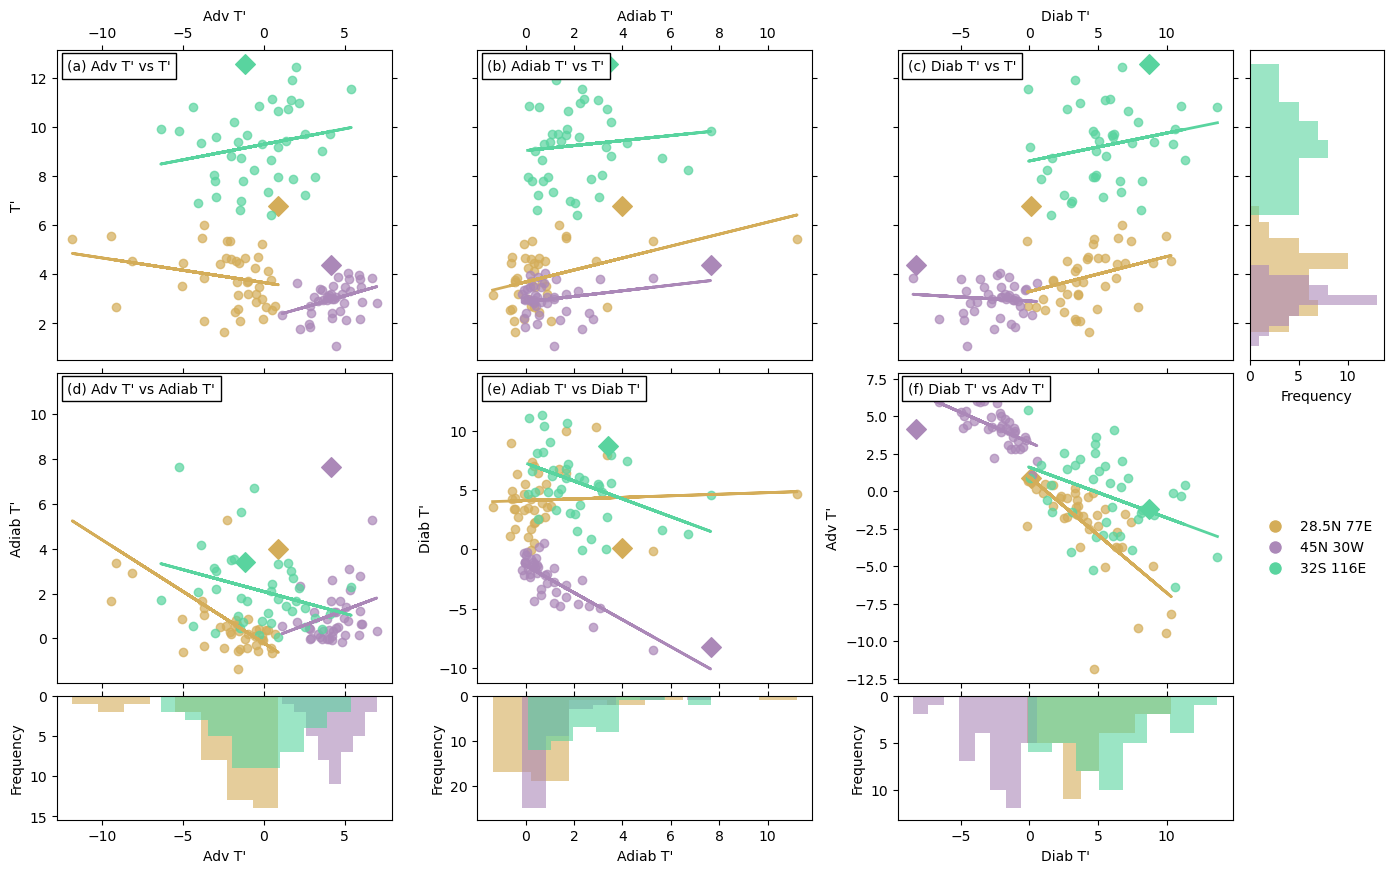
\includegraphics[width=1\linewidth]{images/flat_data} \caption{(a-c) Plots of TX1day $T'$ against the three contributors and (e-f) pair-plots for the contributors for years 1980 to 2020 for three locations. The $T'$ histogram is plotted on the top-right of the figure, and the contributor histograms with 8 bins are plotted below (e-f). The TX1day event acheiving largest $T'$ over the 41 events is plotted as a diamond.}\label{fig:flatdata}
\end{figure}

\section{Trajectory timeseries}\label{trajectory-timeseries}

At every {[}latitude, longitude, year{]} index, the second dataset considers the time-cumulative evolution of the parcel's \(T'\), decomposed into the three contributors. Since each event may have a different genesis-time, all series are padded with zeros before their genesis time, yielding at each location 41 timeseries of length 121 - a trajectory history of 15 days with 3h intervals. The data displays again diverse structures, year-to-year as well as across space. Figure \ref{fig:timeseriesdata} illustrates the year-to-year variability for one example location. Although some repeated structures are found in event \(T'\) and contributor \(T'\)s across years, there are noisy periods and seemingly changing dynamics. For example, the graphs show some trajectories coupling and decoupling in time: the largest TX1day \(T'\) event exhibits advective and diabatic \(T'\) both decreasing until about 2 days before the event, then the diabatic \(T'\) steeply increases while the advective \(T'\) continues to decrease after a brief increase. The same pattern is observed between adiabatic and diabtic \(T'\)s - although with negative correlation - up to 2 days before and then only little association is observed. Some trajectories also exhibit sinusoidal behavior in diabatic \(T'\) with period around 12h (see a number of samples between 10 days to 3 days before the events) which is explained by the day/night variation in solar radiation.

On average, the timeseries exhibit strong auto-correlation with final \(T'\) at small time-lags, decreasing slowly until around 36h after which it cycles between 0.4 and 0.6. Strong auto-correlations are expected since the timeseries consider the accumulation of \(T'\) in time. Advective and adiabatic \(T'\) are poorly correlated with history older than 3 days, while diabatic \(T'\) remains above 0.4.

The cross-correlation between final event \(T'\) and the contributor \(T'\)s is largest and positive for diabatic \(T'\), slowly decreasing over 4 days with a sinusoidal behavior. The only negative correlation is with advective \(T'\) and seems to be largest at longer time-lags. Further timeseries plots for locations chosen in \ref{fig:flatdata} are included in Appendix A.1 and show different characteristics.

\begin{figure}[h]
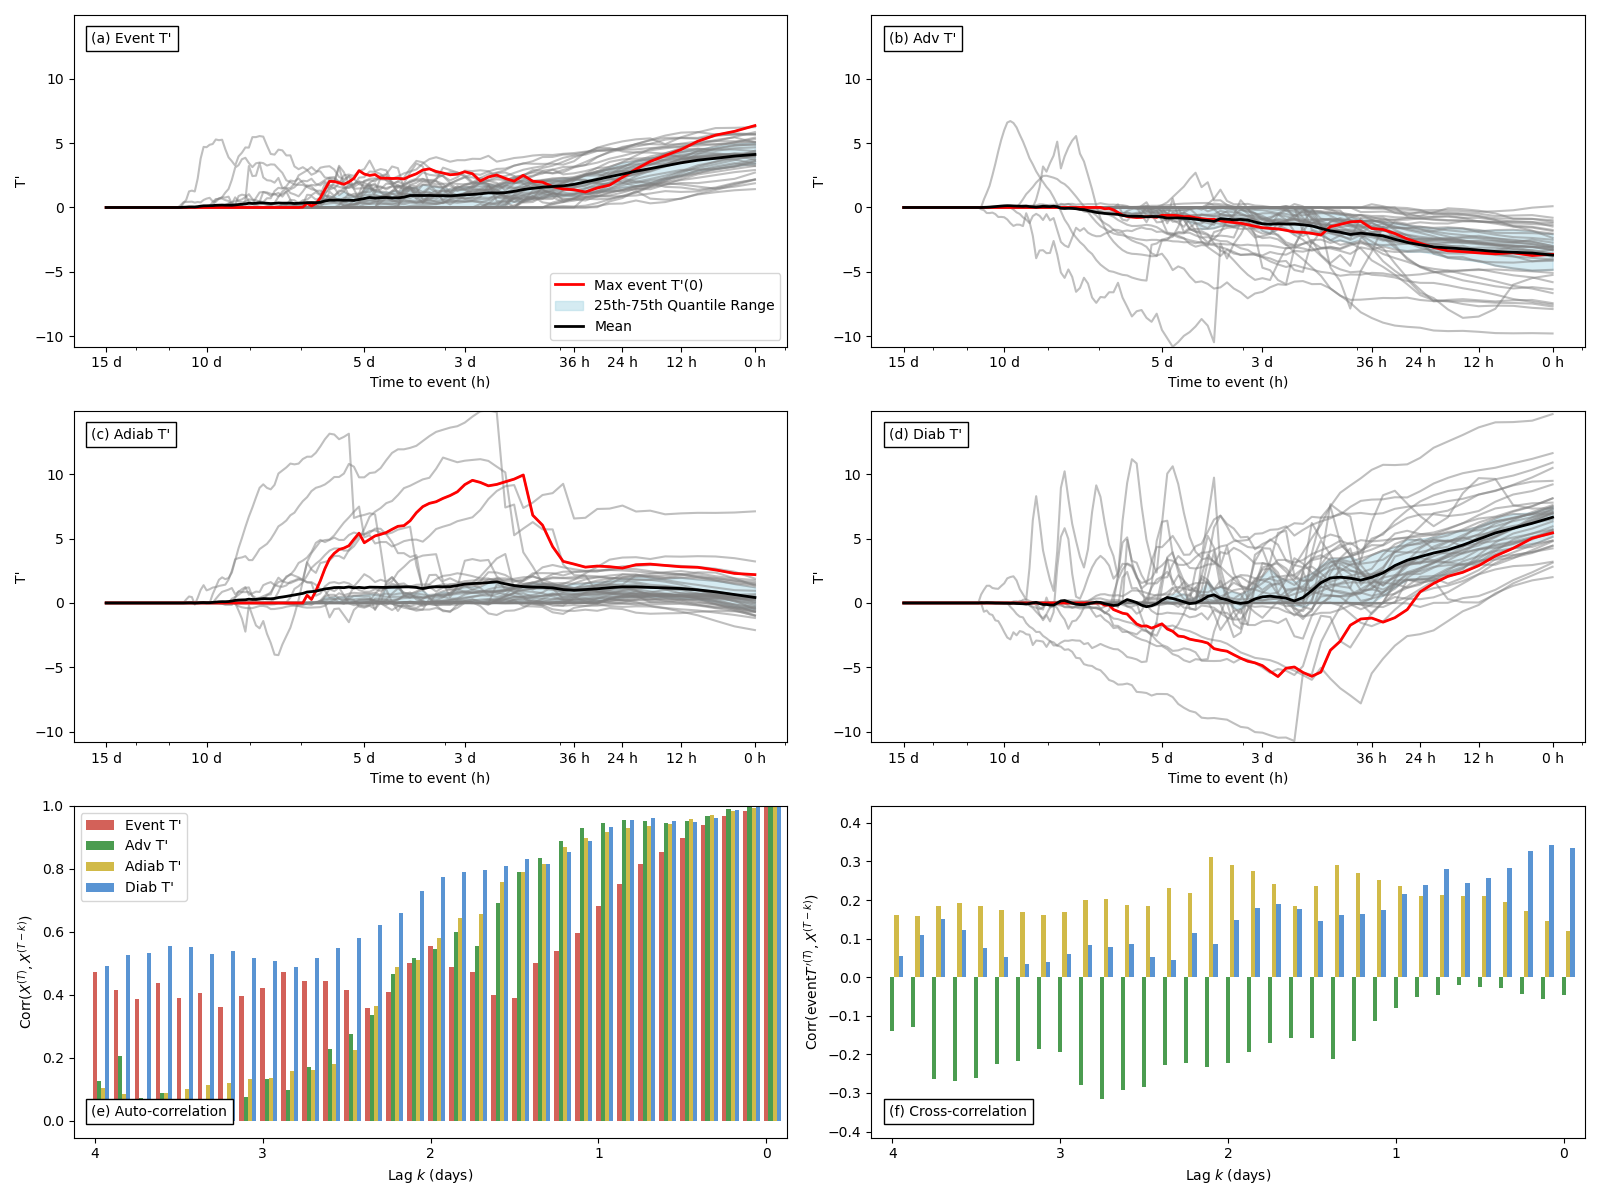
\includegraphics[width=1\linewidth]{images/timeseries_data} \caption{(a-d) Plots of TX1day $T'$ decompositions at 16$^{\circ}$S, 48$^{\circ}$W (vicinity of Brazilia, Brazil) for years 1980 to 2020. The x-axis is logarithmic to better represent the recent history. The trajectory yielding the largest final $T'$ among all years is colored red, the time-mean of all trajectories in black and the inter-quantile range is highlighted in light blue. Plot (e) shows the (auto-)correlation between the final $T'$ and the $T'$ at different lags for the event and each contributor. Plot (f) shows the (cross-)correlation between the final event $T'$ and the $T'$ at different lags for each contributor. They are computed for all samples that have genesis time earlier than the considered time-lag.}\label{fig:timeseriesdata}
\end{figure}

A common approach to reduce auto-correlation in timeseries is compute first-order differences (\((X^{(t)}-X^{(t-1)}\) for time \(t=1,2,...,T\)). However, differenced data in this application has been observed to yield noisy timeseries characterized by many local minima and maxima (see Appendix A.2) as well as considerable remaining auto-correlations. This behavior may hinder the ability of a machine learning model to learn meaningful patterns, and therefore the dataset is not differenced.

\chapter{Statistical methods}\label{statistical-methods}

\section{\texorpdfstring{Variance decomposition of TX1day \(T'\)}{Variance decomposition of TX1day T\textquotesingle{}}}\label{variance-decomposition-of-tx1day-t}

The aim of this thesis is to gain further understanding in the influence of the three \(T'\)-generating mechanisms on TX1day events, particularly relating to the variability in yearly maxima observations. The ideal output of a statistical analysis would then be quantifying the influence of each contributor on a second-moment estimate of yearly maxima TX1day magnitude at each location.

Ranking the influence a certain predictor has on a response relative to other predictors is a common problem in applied statistics. Although \(R^2\) is often reported to provide comparisons of model fit and thus measure the value of certain predictors in explaining the variance of the response, it does not take into account interactions between predictors. Instead, in the context of linear regression models, \cite{lindeman_introduction_1980} - referred to as LMG - propose to quantify predictor importance by computing the average sequential sums-of-squares over all predictor orderings. Averaging over all orderings allows this measure to capture both direct effects and secondary effects of a predictor. \cite{feldman_relative_2005} extended this approach with Proportional Marginal Variance Decomposition (PMVD) that instead considers a weighted average with weights chosen such as to enforce the exclusion criteria - a predictor with zero coefficient is allocated zero importance \citep{gromping_estimators_2007}. \cite{breiman_random_2001}, and extensions thereof, instead propose to measure importance of a predictor by assessing the model's loss of accuracy due to random permutations of the predictor values.

These methods have however been shown to be susceptible to data with highly correlated predictors, as is often the case in observational settings lacking causal assumptions. Furthermore, with many predictors, LMG and PMVD become computationally intensive, as they require computation of \(R^2\) values over all possible orderings. Permutation-based methods scale linearly with the number of predictors but may require running many permutations of each column to output estimates with low variance.

\hyperref[data]{Chapter 3} has indeed demonstrated strong correlations between contributors that are due to inherent physical constraints. In addition, by assuming residuals to be approximately zero, the response and predictors are linearly dependent. This then limits the applicability of standard regression methods and the associated measures of predictor importance that assume them uncorrelated \citep{hooker_unrestricted_2021}. Addressing the constraint that the response is the sum of the three contributors, for example by transforming the contributors to a simplex space \citep{greenacre_compositional_2021}, is also problematic as the data does not follow the positivity constraint: contributions to \(T'\) may be negative. Pre-processing the data to enforce positivity leads to poor representation of the domain and hinders interpretation. Furthermore, more robust scale measures - such as truncated variance - would not be appropriate as information of tail events that are often associated with the largest human impact needs to be preserved.

Then, to extend the first-moment characterization of TX1day events by \cite{rothlisberger_quantifying_2023}, we propose a variance decomposition of \(T'\) that quantifies the contributions of physical processes to variability. Recall that computation of \eqref{eq:tdecomp} gave rise to residuals that may be assumed zero. Then the final \(T'\) of the event is related linearly to the \(T'\) generated by the three processes with a bias from the seasonality term, which is is generally small. Then, for \(n\) independent events achieving temperature anomalies \(\{ T' \}_{1:n}\), data is described by \({T'}_i \approx \text{adv}_i +\text{adiab}_i +\text{diab}_i\) and therefore:

\begin{equation}
   V(\{ T' \}_{1:n}) \approx \sum_{c \in \{\text{adv},\text{adiab},\text{diab}\}} V(\{ c \}_{1:n} ) + \sum_{c, d \in \{\text{adv},\text{adiab},\text{diab}\} , c\neq d} \text{Cov}(\{ c \}_{1:n} ,\{ d \}_{1:n})
\label{eq:vardecomp}
\end{equation}

For further support, a brief background on variance and associated estimates is presented in Appendix B.

Applying \eqref{eq:vardecomp} to every location on Earth yields a direct and systematic approach to the analysis of global patterns of hot extreme variability, while the presence of complex dependencies between physical processes is explored by the contributions from covariance terms. The linearity of the covariance operator and the fact that it is un-normalized, in comparison to correlation for instance, allows for an intuitive comparison of second-moment contributions. We argue that considering the variance of the contributors without adjusting for the influence of other contributors due to existing correlation is more informative. For example, a large variation in adiabatic \(T'\) contribution is important to report, regardless of the additional influence of advective and diabatic processes; if the sum of adiabatic and advective \(T'\) has small variance, it will be reflected in a negative covariance between the contributors. The limitation of using an un-normalized quantity is the fact that a large mean magnitude will in most cases imply a larger variance. Therefore, meaningful interpretation of second-moment estimates will also require consideration of first-moment estimates.

To summarize the spatial structure of TX1day \(T'\) variance and its decomposition, variance terms will be ranked with respect to their magnitude according to the following definition (applied to both mean and variance decomposition data): a contributor is dominant if it is at least twice as large as the second largest contributor; two contributors are dominant if they are both at least twice as large as the remaining contributor; else, no contributor is dominant. As both mean and variance decompositions are additive, this importance definition allows for a intuitive comparison. Covariance terms are omitted in these comparisons as they are observed to be generally more negative than the variance terms, except in few exceptions.

\section{Principle Component Analysis of contributors}\label{principle-component-analysis-of-contributors}

As discussed, strong inter-contributor correlations limit the interpretability of the variance decomposition, but are important in understanding the physical mechanisms associated with hot extreme development and their constraints. To characterize the dependence structure between the contributors, Principal Component Analysis (PCA) is employed to assess the degrees of freedom of the heat-generating systems and provide an alternative importance definition to rank the contributors at each location.

PCA - known as Empirical Orthogonal Functions in climate sciences - is a linear transformation introduced by \cite{pearson_liii_1901} and first applied in climate sciences for weather prediction by \cite{lorenz_empirical_1956}. It is commonly used as a dimension reduction method - to obtain a low-dimensional representation of high-dimensional inputs - and in identifying and quantifying modes of variability such as the North-Atlantic Oscillation and the ENSO. The PCA problem consists in finding a projection \(\mathbf{f}(\mathbf{x})\) that yields lower dimensional and orthogonal representations of the data that retain the most information.

Given \(n\) mean-centered samples \(\mathbf{X} = (\mathbf{x}_1, ..., \mathbf{x}_n) \in \mathbb{R}^{n \times p}\) of dimension \(p\), the solution to obtain PCA transformation \(\mathbf{W} = (w)_{ij} \in \mathbb{R}^{p \times l}\) for \(1 \leq l \leq p\) and \(l-\)dimensional representations called PC scores \(\mathbf{z}_1, ..., \mathbf{z}_{n} \in \mathbb{R}^l\) is given by:
\begin{equation}
(\mathbf{W}, \mathbf{z}_1, ..., \mathbf{z}_{n}) = \argmin_{\mathbf{W}^{\intercal}\mathbf{W}=\mathbf{I}_l,\mathbf{z}} \, \sum_{i=1}^n \left|\left| \mathbf{z}_i  \mathbf{W}^{\intercal}- \mathbf{x}_i \right|\right|^2_2
\label{eq:pcatrans}
\end{equation}

with \(f(\mathbf{x}_i) = \mathbf{z}_i = \mathbf{x}_i \mathbf{W}\). The unit column vectors \(\mathbf{w}_{\bullet 1}, ...,  \mathbf{w}_{\bullet l}\) are related to the empirical covariance matrix \(\boldsymbol{\Sigma}\) of \(\mathbf{X}\) as they are its eigenvectors corresponding to its eigenvalues \(\lambda_{(1)}, ..., \lambda_{(p)}\) ranked in decreasing magnitude:
\begin{equation}
\boldsymbol{\Sigma} = \sum_{i=1}^p \lambda_{(i)} \mathbf{w}_{\bullet i} \mathbf{w}_{\bullet i}^{\intercal} 
\label{eq:pcacov}
\end{equation}

The first PC (PC1) then points in the direction with the largest variance, PC2 points in the direction orthogonal to PC1 with the largest residual variance, etc. The proportion of variance explained by a single PC can be computed using the eigenvalues:
\begin{equation}
\text{\% explained variance }(\text{PC}i) = \frac{\lambda_{(i)}}{\lambda_{(1)}+...+\lambda_{(p)}}
\label{eq:pcaexplvar}
\end{equation}

Untruncated PCA is then applied to the advective, adiabatic and diabatic \(T'\) contributions of the 41 events at each location. To present an alternative measure of importance than the variance decomposition, each contributor is centered and scaled independently. This focuses the analysis on the contributor dependencies since it compares the variability structure without the influence of absolute magnitudes. The components are computed exactly using Singular Value Decomposition as proposed by \cite{halko_finding_2011} and the analysis will consider the proportion of explained variance for each PC and relate the resulting directions of the PCs to the contributors.

Additionally, at each location we have three PC directions - i.e.~the unit column vectors \(\mathbf{w}_{\bullet 1}, \mathbf{w}_{\bullet 2},  \mathbf{w}_{\bullet 3}\) - that point in the orthogonal directions of largest variability. To represent these new axes at every location, we partition them in 7 categories, similarly to the dominance definition introduced in \hyperref[variance-decomposition-of-tx1day-t]{4.1}. Since the directions are unit-vectors in 3D space, the vector created by applying element-wise absolute-value lies on the positive octant of the surface of a unit sphere. This surface is partitioned into three corner regions (each contributor), the center (combination of all contributors) and three remaining surface divided evenly (pair-combinations), according to figure \ref{fig:pcascores}.

\begin{figure}[h]

{\centering 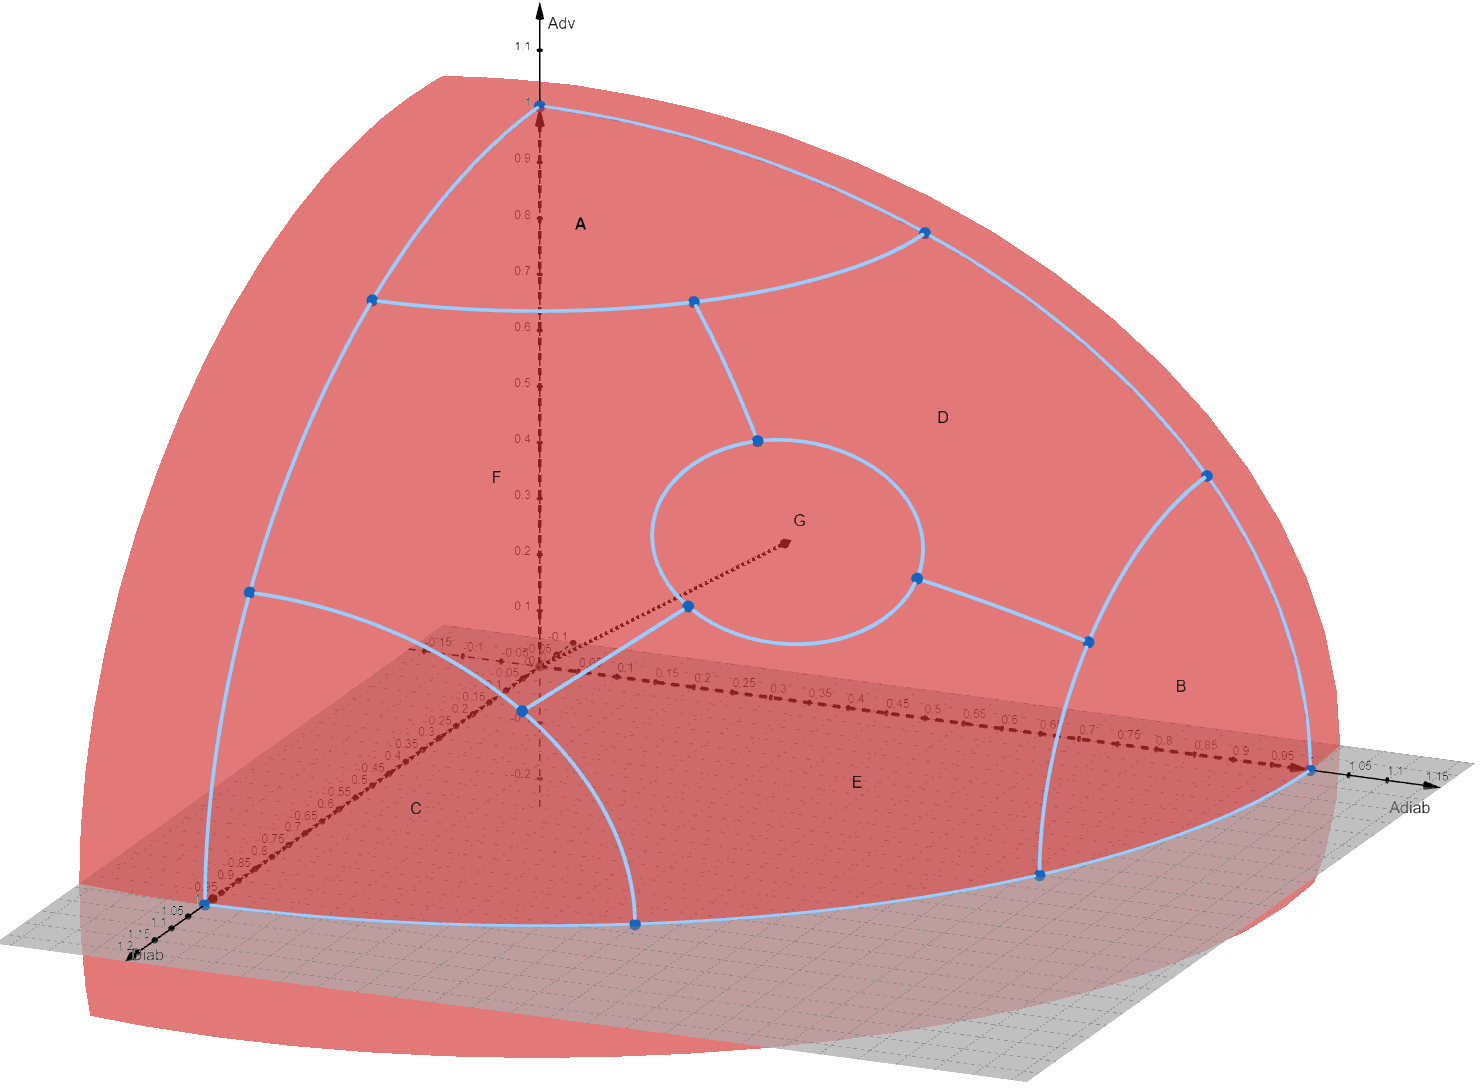
\includegraphics[width=0.8\linewidth]{images/pca_partition} 

}

\caption{Illustration of the partitioning of surface of PC absolute-value vectors into 7 categories: advective (A), adiabatic (B), diabatic (C), advective-adiabatic (D), adiabatic-diabatic (E), diabatic-advective (F) and all (D). The construction points all lie on planes parallel to the axes at values $\sqrt{2}/2$, $0.5$ and $\sqrt{3}/2$ that correspond to 30, 45 and 60$^\circ$ angles between the axial planes.}\label{fig:pcascores}
\end{figure}

Finally, PCA is preferred over machine-learning approaches because of the small sample sizes at each location, it is variance-based and therefore can be related to previous work, and has an intuitive interpretation.

\section{Forecasting TX1day contributor trajectories}\label{forecasting-tx1day-contributor-trajectories}

Considering final \(T'\) is useful for quantifying the cumulative contributions of physical processes to hot extreme events, as well as investigate the overall dependence patterns between them. To extend this analysis and provide a more precise assessment of the behavior of physical processes in the development of hot extreme events, we consider trajectory information. The added temporal structure allows the investigation of the underlying dynamics. For example, rapid \(T'\) growth of a certain physical process in the final day before an extreme event can be distinguished from a gradual gain that was previously reported as a single cumulative total. Understanding the timescales of advective, adiabatic and diabatic \(T'\) growth are particularly important for the development of warning systems in face of increasingly dangerous hot extreme events.

Trajectory-based analyses in hot extreme research are often carried out case-by-case. We propose leveraging the flexibility of Deep-Learning (DL) models to investigate the predictability of yearly maxima TX1day \(T'\) decomposition trajectories on a global scale. In this setting, a model is trained to forecast advective, adiabatic and diabatic \(T\) in the final period of trajectory given their past. A model that performs adequately can then be assumed to have learned meaningful patterns in the data that reflect the true dynamics of the system. Then, the model can be analysed to determine the contributors and time-windows that most affect the prediction, thus unraveling temporal interactions of the physical mechanisms in the development of hot extreme events. Before introducing the model employed in this thesis, we give a brief overview of machine learning.

Machine learning and in particular DL architectures have recently received a lot of attention in atmospheric and climate sciences due to their performance in modelling complex high-dimensional systems and their computational efficiency in comparison to numerical weather prediction. DL models have largely been used to develop weather forecasting models \citep[see for example][]{srivastava_weather_2022} and to learn parameterizations from simulated and observational datasets \citep{barahona_deep_2023}. We first provide a brief introduction to a DL architecture that has been used extensively in timeseries applications.

Supervised DL involves the parameterization of arbitrarily complex functions - called networks - and estimation of these parameters by propagating input data through the network and evaluating the outputs' accuracy against the given truth - called the loss. By using a differentiable loss and network, the parameters can be updated. With sufficient data and learning iterations, the model parameters will be progressively updated to improve accuracy.

The modelling and processing of sequential data requires specific architectures such as Recurrent Neural Networks (RNNs) that can leverage sequential dependencies to learn representations of the underlying dynamical system. At a high level, RNN function by iteratively processing each time-step to update a set of hidden weights that retain memory - a memory cell. However, standard implementations have been shown to suffer from vanishing gradients - when parameter updates approach zero due to decaying gradient magnitudes, thus impeding learning - in applications with long-term temporal dependencies \citep{noh_analysis_2021}.

Long Short-Term Memory (LSTM) networks \citep{hochreiter_long_1997} were the first extension of RNNs introduced to solve vanishing gradients. They contain a memory cell that is modulated by other units - called gates - to learn to determined when to `forget' information. More formally, an LSTM memory cell is composed of hidden states \(H\), cell states \(C\) and four gates: the input, forget, cell and output gates. Given a sequence of data, a memory cell recurrently propagates a data sequence one timestep at a time to update the gate, hidden and cell parameters. Given some initial hidden \(H^{(t-1)}\) and cell states \(C^{(t-1)}\), an input \(x^{(t)}\) at time-step \(t\) is processed according to:
\begin{equation}
  \begin{aligned}
  \text{Gating:} \quad & \\
    i^{(t)} &= \sigma \left( W_{ii} x^{(t)} + b_{ii} + W_{hi} H^{(t-1)} + b_{hi}  \right) \\
    f^{(t)} &= \sigma \left( W_{if} x^{(t)} + b_{if} + W_{hf} H^{(t-1)} + b_{hf}  \right) \\
    g^{(t)} &= \tanh \left( W_{ig} x^{(t)} + b_{ig} + W_{hg} H^{(t-1)} + b_{hg}  \right) \\
    o^{(t)} &= \sigma \left( W_{io} x^{(t)} + b_{io} + W_{ho} H^{(t-1)} + b_{ho}  \right)
  \end{aligned}
\label{eq:lstm1}
\end{equation}

\begin{equation}
  \begin{aligned}
  \text{Memory update:} \quad & \\
    C^{(t)} &= f^{(t)} \ast C^{(t-1)} + i^{(t)} \ast g^{(t)} \\
    H^{(t)} &= o^{(t)} \ast \tanh \left( C^{(t)}\right)
  \end{aligned}
\label{eq:lstm2}
\end{equation}

where \(\sigma\) and \(\tanh\) are the sigma and tanh activation functions; \(\ast\) represents element-wise multiplication; \(W_{ij}\) and \(b_{ij}\) are matrices of learned weight and bias parameters for the input (\(j=i\)) and the hidden states (\(j=h\)); \(i^{(t)},f^{(t)},g^{(t)}\) and \(o^{(t)}\) are the forget, input and output gates at time \(t\), respectively. A schematic representation can be found in Figure \ref{fig:lstm}.

\begin{figure}[h]

{\centering 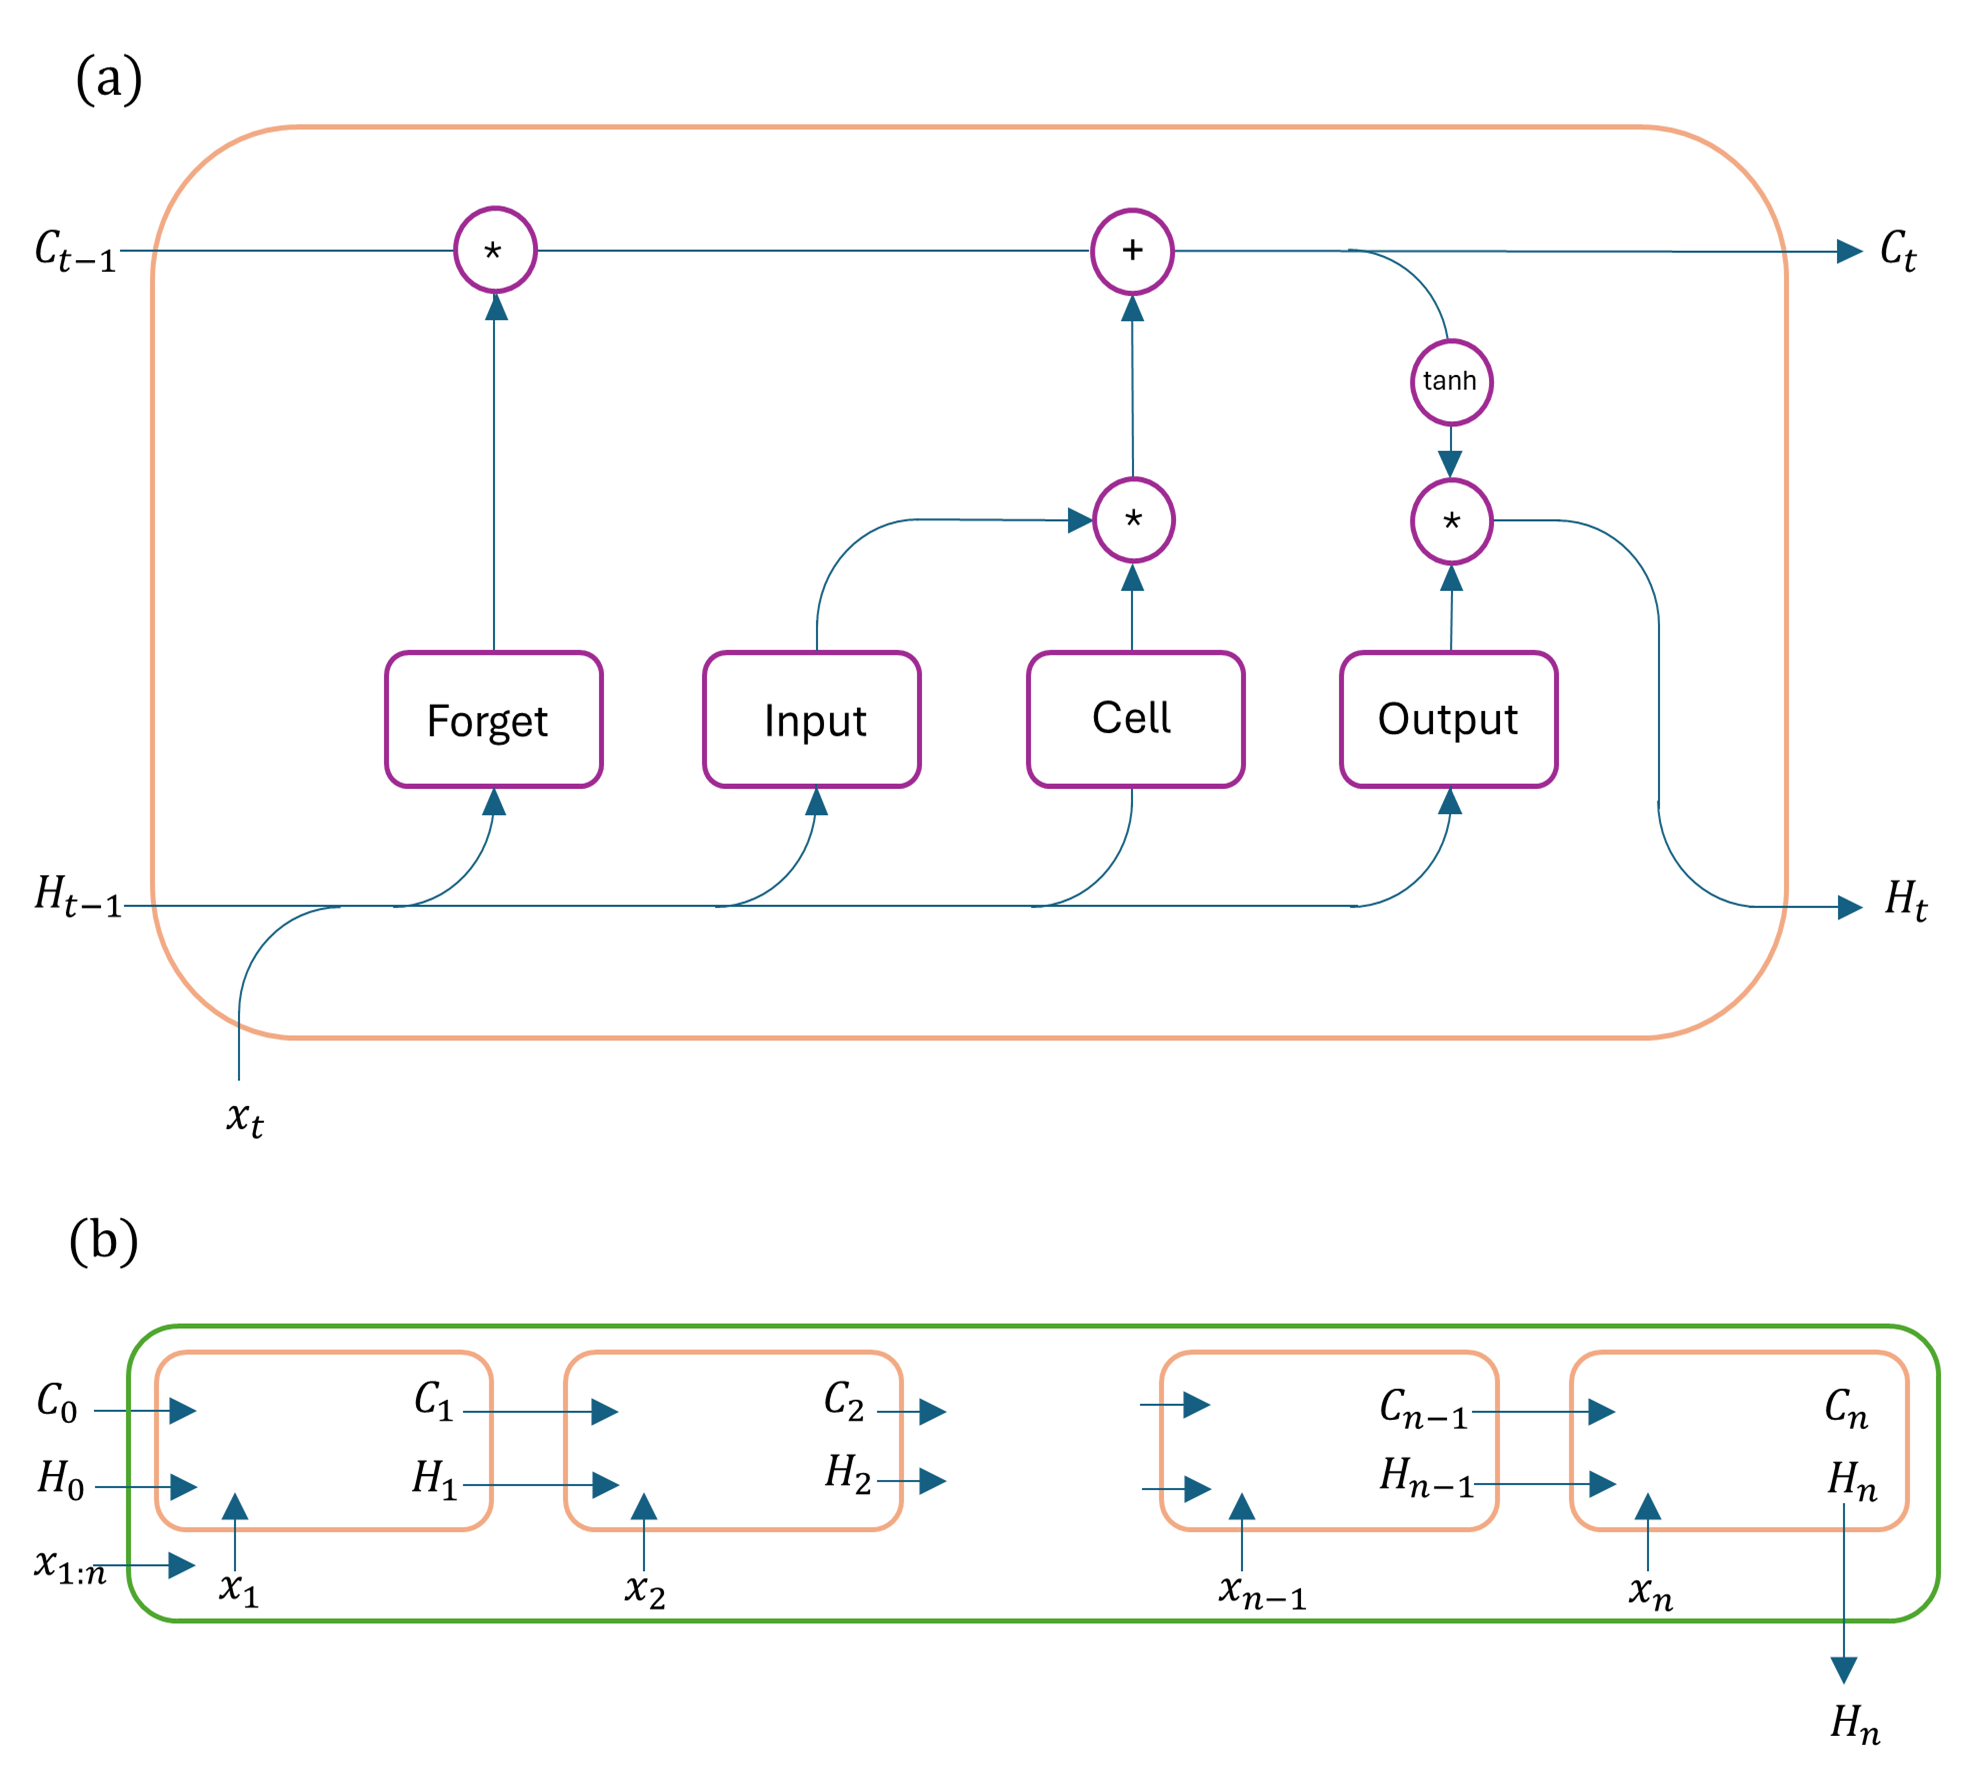
\includegraphics[width=0.8\linewidth]{images/lstm_fig} 

}

\caption{(a) Representation of an LSTM memory cell (in orange) that, given intitial hidden states $H^{(t-1)}$, cell states $C^{(t-1)}$ and input $x^{(t)}$, outputs the updated hidden $H^{(t)}$ and cell $C^{(t)}$ states. Purple shapes represents operations: $\ast$ matrix multiplication, $+$ element-wise addition, tanh the tanh activation function, and the Forget, Input and Output gates are as define in equations 4.5. (b) The same LSTM cell but unfolded. For an input of initial hidden states $H^{(0)}$, cell states $C^{(0)}$ and data sequence $x^{(1:T)}$, it outputs final hidden states $H^{(T)}$ that can then be further processed (e.g. by a fully connected layer).}\label{fig:lstm}
\end{figure}

LSTM layers, composed of a number of memory cells, may used in different ways depending on the data structure and task at hand. In timeseries forecasting applications, most models use the final hidden states \(H^{(T)}\) of the last LSTM layer as lower-dimensional feature representations of every input that are then further processed by one or more fully-connected NN layers. There is a rich and evolving literature on LSTM-based architectures and LSTM variants and thus refer the reader to comprehensive review papers such as \cite{hu_time_2020} and \cite{han_review_2021}.

Here, a global LSTM-based DL model is trained to forecast the final 8 timesteps (1 day) of each contributor of the TX1day event decomposition trajectories given their history. The model is composed of a single LSTM layer and a linear output layer to process the final hidden states \(H^{(T)}\) into 24 outputs (3 variables x 8 timesteps). The rich diversity of timeseries behaviors and patterns as well as the occurrence of anomalous large negative and positive values motivates careful design of the optimization procedure.

First, the three contributors in the training data are centered by the global median and scaled according to the global interquartile range, as these quantities are more robust than the mean and variance and scaling has been shown to stabilize training. Second, the model is trained with stochastic gradient descent. Although this is computationally less efficient than mini-batch gradient descent for such large training datasets, initial tests showed vanishing gradients when using batches leading to constant forecasts. Third, the Huber-loss is employed to leverage the benefits of the mean-squared-error and mean-absolute-error loss: improved stability near zero and decreased sensitivity to extreme values, respectively. The Huber-loss threshold is set to its typical value 1. Fourth, generalization is improved by using L2-regularization that has been shown to be particularly beneficial for prediction tasks on multivariate time series \citep{zhou_explore_2019}. It penalizes the magnitude of model weights to ensure that the resulting function is less sensitive to small perturbations, thus limiting over-fitting. Fifth, a dropout layer is introduced between the LSTM and fully connected layers to further promote model generalization.

Then, given network output \(\mathbf{\hat{y}} = (\mathbf{\hat{y}}_{\text{adv}}, \mathbf{\hat{y}}_{\text{adiab}}, \mathbf{\hat{y}}_{\text{diab}})\) and truth \(\mathbf{y} = (\mathbf{y}_{\text{adv}}, \mathbf{y}_{\text{adiab}}, \mathbf{y}_{\text{diab}})\), model parameters \(\mathbf{W}\), the L2-regularization hyper-parameter \(r\) and Huber-loss threshold \(\delta\), the objective function is given by:

\begin{equation}
  \begin{aligned}
   \text{obj}(\mathbf{\hat{y}},\mathbf{y}) & = \frac{1}{24}\sum_{i=1}^{24} l(\hat{y}_i,y_i) + r \cdot || \mathbf{W} ||_2 \\
   l(\hat{y},y) & = \begin{cases} 0.5(y - \hat{y})^2, & \text{ if } |y - \hat{y}| < \delta \\
   \delta \left( |y - \hat{y}| -0.5\delta \right), & \text{ otherwise } \end{cases}
   \end{aligned}
\label{eq:obj}
\end{equation}

where \(||\cdot ||_2\) is the L2-norm and \(l_i\) the Huber-loss for one prediction.

\begin{figure}[h]

{\centering 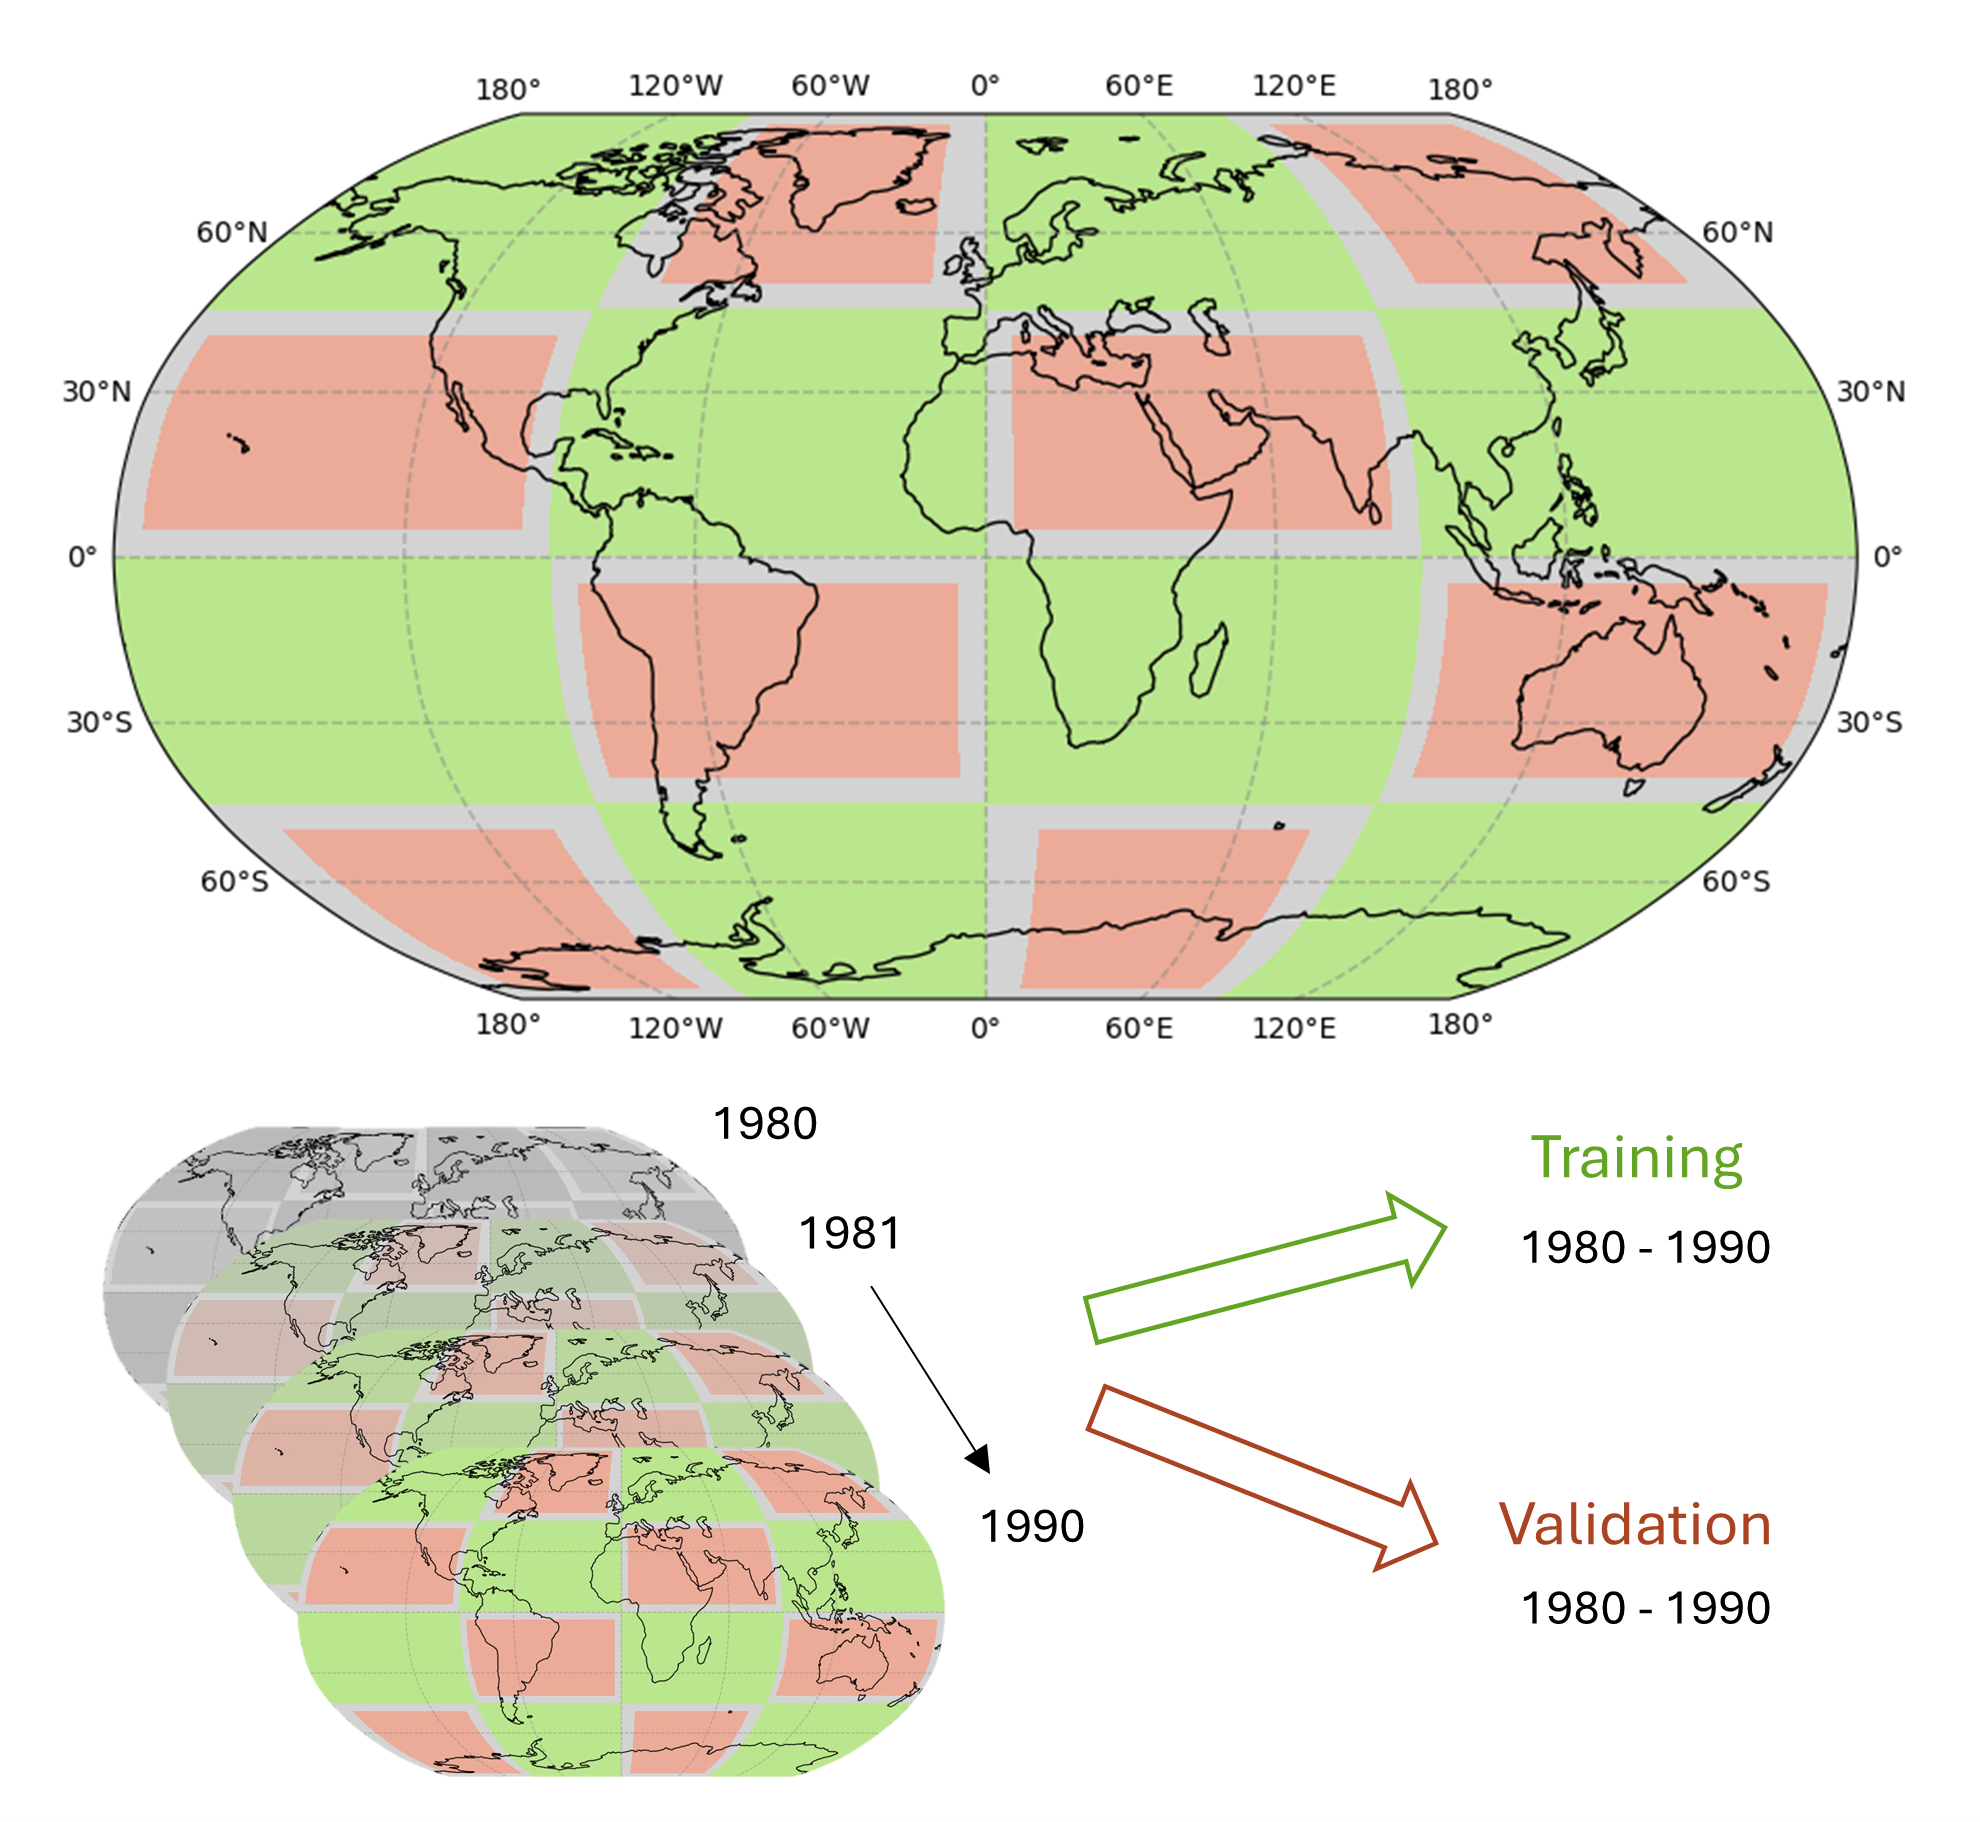
\includegraphics[width=0.8\linewidth]{images/test_train_fig} 

}

\caption{Training and validation splitting scheme. Years between 1980 and 2000 are used for training (green shaded areas) and validation (red shaded areas). The remaining years 2001 to 2020 and the whole globe are used for inference.}\label{fig:traintest}
\end{figure}

Due to the high-resolution of ERA5 data, the dataset contains over 10 million timeseries. To select the model hyper-parameters (L2-regularization weight, LSTM hidden unit size), the globe is divided into 16 rectangular regions according to figure \ref{fig:traintest}: 8 for training, 8 for validation. In addition, the timeseries exhibit large spatial dependencies within a given year since they may share the same flow. Therefore, to have a more faithful estimation of generalization performance, the validation regions are reduced in latitude and longitude extent by a factor proportional to the maximum of the average trajectory distance in each region. Finally, to limit computational burden and perform inference on unseen data everywhere on the globe, only years from 1980 to 1990 are used for training.

The final model parameters are obtained by randomly sampling 50'000 timeseries (\(\sim 4\%\) of all training data) and training a model instance for each combination of LSTM layer hidden unit size \([48,64,88]\) and L2-regularization weight \([0,10^{-6},10^{-4}]\). An estimate of generalization loss is computed on half of the validation data, randomly sampled. Each instance is trained with the Adam algorithm \citep{kingma_adam_2017}, a learning rate of \(2\times 10^{-4}\) and for a maximum of 15 epochs, stopped early if validation loss does not improve within three epochs. LSTM hidden and cells states are re-initialized at every input with zero matrices. The parameters of the final model are chosen by considering low validation loss (see Appendix C.1 for results) relative to model complexity and expected behavior on a larger dataset. The final model is trained on the full training data and is used to forecast each test timeseries, consisting of all locations for years 1991 to 2020. To obtain a reference predictive performance, a simple constant model is created that outputs the latest input value for each contributor - i.e.~the value at time 27h before the event.

\chapter{Results}\label{results}

\section{\texorpdfstring{Relating TX1day \(T'\) variability to component variability}{Relating TX1day T\textquotesingle{} variability to component variability}}\label{relating-tx1day-t-variability-to-component-variability}

The variance decomposition on 40 years of ERA5 data reveals large spatial diversity in year-to-year TX1day variance (Figure \ref{fig:vardecomp}). As anticipated, the patterns closely resemble those of the mean of TX1day magnitudes in \citep{rothlisberger_quantifying_2023}, since the variance is un-normalized and therefore scales with magnitude. There is a strong ocean-land contrast, with low variances in the order of 2 K\(^2\) over oceans and mostly above 4 K\(^2\) over land. A general trend over land is the increase in variability further from the Equator. There exists nonetheless important exceptions: the West coasts of North America, West coasts of Southern Chile, South-western coasts of Australia and the West coasts between Mauritania and Northern Europe all exhibit large TX1day variability, while tropical land such as the Amazonia, South-east Asia and Indonesia, equatorial Africa and parts of the Eastern Saharan show low variability compared to the oceans. The largest peaks of variability occur in the bay of the Antarctic Peninsula and an oceanic hot spot centered at 70° S 160° W, as well as relatively large hotspots in the coastal regions described above.

Individual contributors have mostly larger variance and vary spatially with no single contributor dominating globally. The advective and adiabatic \(T'\) variance have similar spatial distribution over land, while they seem to complement each other over oceans with large adiabatic \(T'\) variance in the extra-tropics and large adiabatic \(T'\) variance in the sub-tropics. Key hotspots of very large variance for both contributors include regions of high topography (particularly over Rockies, the Andes and the Himalayas) as well as the Arctic and Antarctic ice sheets, with values mostly above 32 K\(^2\) and 64 K\(^2\) respectively. In comparison, the variances of diabatic \(T'\) are more uniform with a less pronounced ocean-land contrast, and are particularly small over oceans east of the continents at the Equator with values between 0 and 2 K\(^2\). The storm track regions, especially the upstream portions of the NH, have larger advective \(T'\) variance than the surrounding oceans, which resembles the TX1day variance map.

Covariances between contributors are predominantly negative and again display diverse spatial patterns. The covariances between advective and adiabatic \(T'\) are positive only over the extra-tropical oceans; between advective and diabatic \(T'\) over small regions in the tropical oceans and the Greenland and Antarctic ice sheets; between diabatic and adiabatic \(T'\) over regions of high topography and within the African and Australian continents. Over oceans, the covariance between advective-adiabatic and advective-diabatic complement each other with positive and negative contributions, while the covariance between diabatic and adiabatic \(T'\) is almost always negative.

Spatial patterns in mean magnitude of contributors mainly agree with those in the variance over land, but not over the oceans. The advective \(T'\) patterns are most different on the coast of Western North-America, coastal North-western Africa and the ocean region West of Australia. The diabatic \(T'\) patterns are the most different, in particular over Southern hemisphere oceans, where the mean patterns show much stronger latitudinal gradient and miss important large-variance regions on the west of the continents. The adiabatic \(T'\) patterns instead shows good agreement over the oceans, while some differences exist in the Sahara, eastern North-America and the storm tracks, both in the Northern and Southern hemispheres.

\begin{figure}[h]
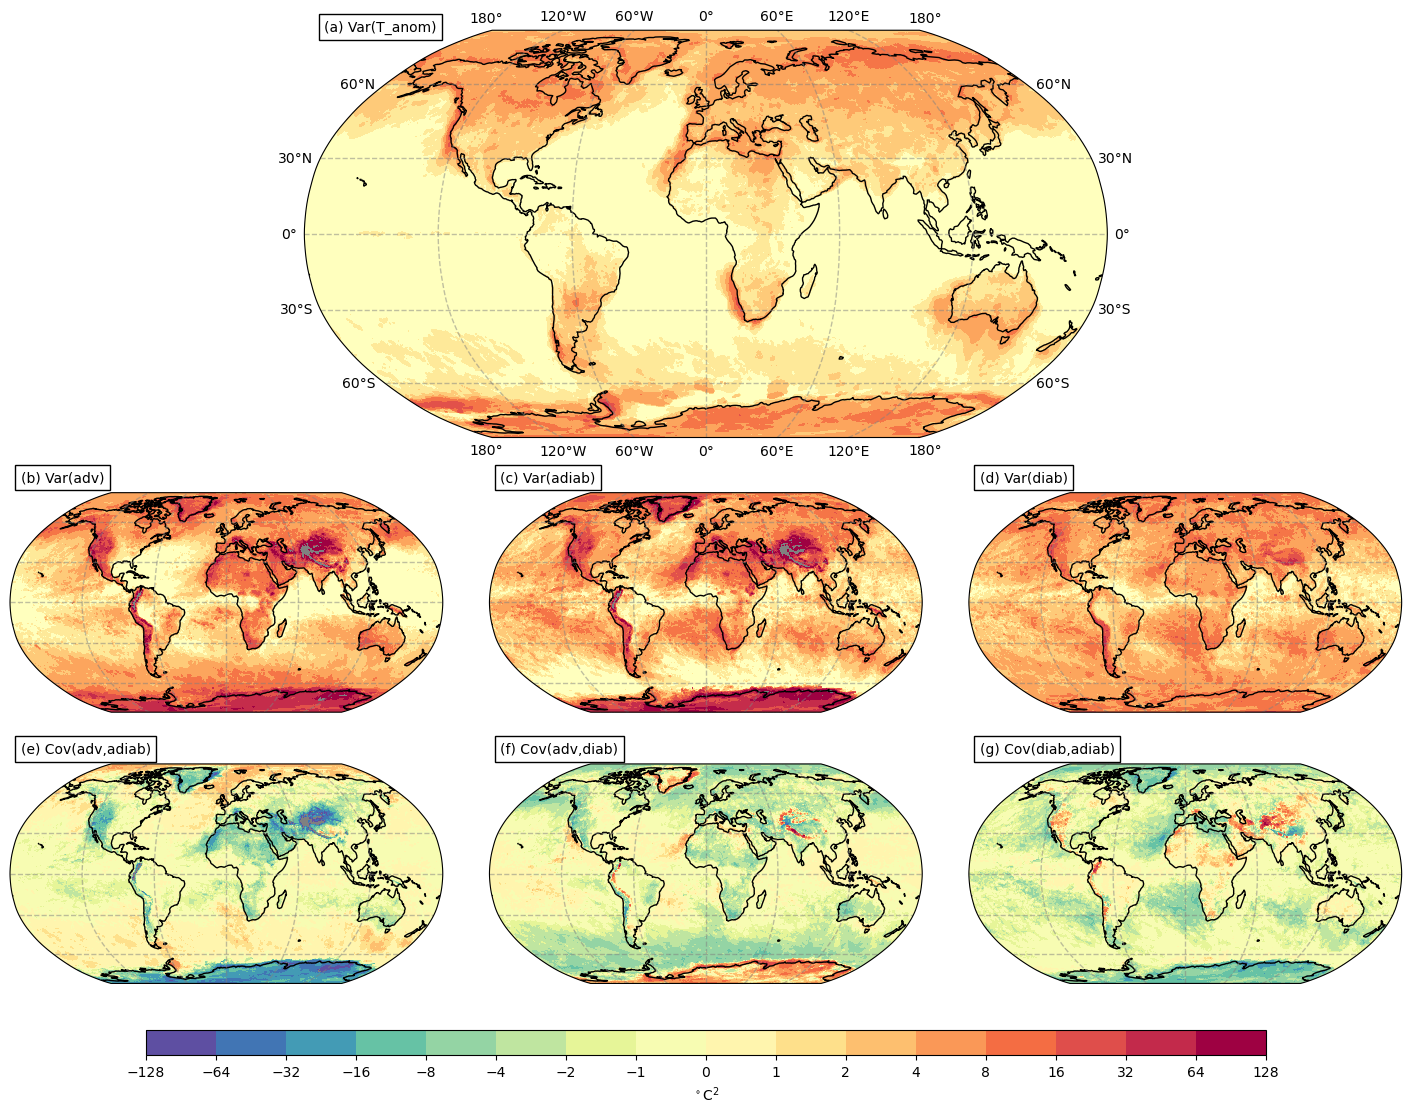
\includegraphics[width=1\linewidth]{images/vardecomp} \caption{(a) Variance of TX1day series decomposed into (b) variance of advective $T'$, (c) adiabatic $T'$, (d) diabatic $T'$, and the the covariances between the contributors (e,f,g). Grid points with very high variances or covariances magnitudes (below -128 and above 128, corresponding to less than 0.6\% of all observations) are colored grey.}\label{fig:vardecomp}
\end{figure}

Similarly to mean-characteristics, the ocean-land contrasts in TX1day variance can be explained by water's larger heat capacity, since a slower temperature gain by solar radiation limits the short-term gain in temperature of a parcel. This is supported by a more uniform diabatic \(T'\) variance over oceans and suggests that cloud cover can influence \(T'\) growth particularly at the end of TX1day event trajectories when parcels are close to the ocean surface. Regions of larger variance over oceans - in TX1day \(T'\) and all contributors - are found near the coasts and can be attributed to trajectories that predominately evolve over land and therefore involve more variable heat-generating mechanisms.

For example, the variability hotspot located on North-Western African coast involves the typical summer-time Azores high-pressure system inducing trade winds from North and the Saharan low-pressure system inducing the Harmattan winds that originate from the continent \citep{adame_saharan_2022}, converging on the Moroccan coast and travelling in a South-westerly direction along the coast. Yearly variability in this synoptic situation can then lead to changes in the contributions from trade winds or Harmattan winds, that evolve very differently.

The mean decomposition showed large cancellation between contributors in many regions. The generally large and negative covariances supports this fact. Furthermore, these regions tend to exhibit large variance in both/either/one of the contributing processes. The Northern and Southern Hemisphere storm tracks have large mean positive contributions from advective \(T'\) with large dampening by diabatic \(T'\), while small but positive contributions from adiabatic \(T'\). This study confirms that observed variability in the TX1day \(T'\) is impacted both by variability in these competing mechanisms, but additionally finds moderate contribution from adiabatic \(T'\) and the covariance between advective and adiabtic \(T'\) in the upstream portion of the storm tracks, that has previously been neglected. This observation is also noted in Easten Brazil, continental southern Africa, Australia and the northern East coast of North America - although with diabatic \(T'\) and advective \(T'\) contributing positively and negatively in the mean, respectively. This is highly significant since changes in variability of hot extremes under climate change may not only be influenced by changes in mean-dominant physical processes, but also those that affect second-moment characteristics, supporting work by \cite{simolo_quantifying_2022}.

Assessing the variability in these dampening mechanisms, or attributing importance of the positive or negative contributor, is difficult without considering the temporal evolution of these interactions. However, the spatial patterns in the covariance between the contributors is then a useful tool in determining regions where competing effects are present and influence the observed variability of resulting TX1day events. Furthermore, the diversity in covariance patterns is suggestive of complex and sensitive TX1day events.

\section{\texorpdfstring{Comparing contributions to TX1day \(T'\) mean and variance}{Comparing contributions to TX1day T\textquotesingle{} mean and variance}}\label{comparing-contributions-to-tx1day-t-mean-and-variance}

Figure \ref{fig:dominant} maps the most important contributor/s - according to to the definition introduced in \hyperref[variance-decomposition-of-tx1day-t]{Methods} - for the mean \citep{rothlisberger_quantifying_2023} and variance decompositions to more concisely compare their differences.

In most oceanic and subtropical land, advective and/or adiabatic \(T'\) dominates the mean while the variance is characterized additionally by significant contribution from diabatic \(T'\). This is highlighted in the Northern and Southern Hemisphere storm tracks. In remaining regions with mean-dominating diabatic \(T'\), the variance of TX1day \(T'\) is dominated by diabatic \(T'\) and most often advective \(T'\) - such as in Equatorial Africa, Eastern South America, Western Australia and Eastern India. In fact, only few regions have a single dominating contributor in the variance. The North-western African, South-western African and Western North-american coasts, a large part of the Mediterranean and the tropical Pacific are dominated by adiabatic processes. Small regions in the Amazonia, Western equatorial Africa and small regions south of the Northern Hemisphere storm tracks are dominated by diabatic processes. Finally, the upstream portion of the Northern Hemisphere storm tracks and a small coastal band around the Antarctic are dominated by advective processes.

\begin{figure}[ht]
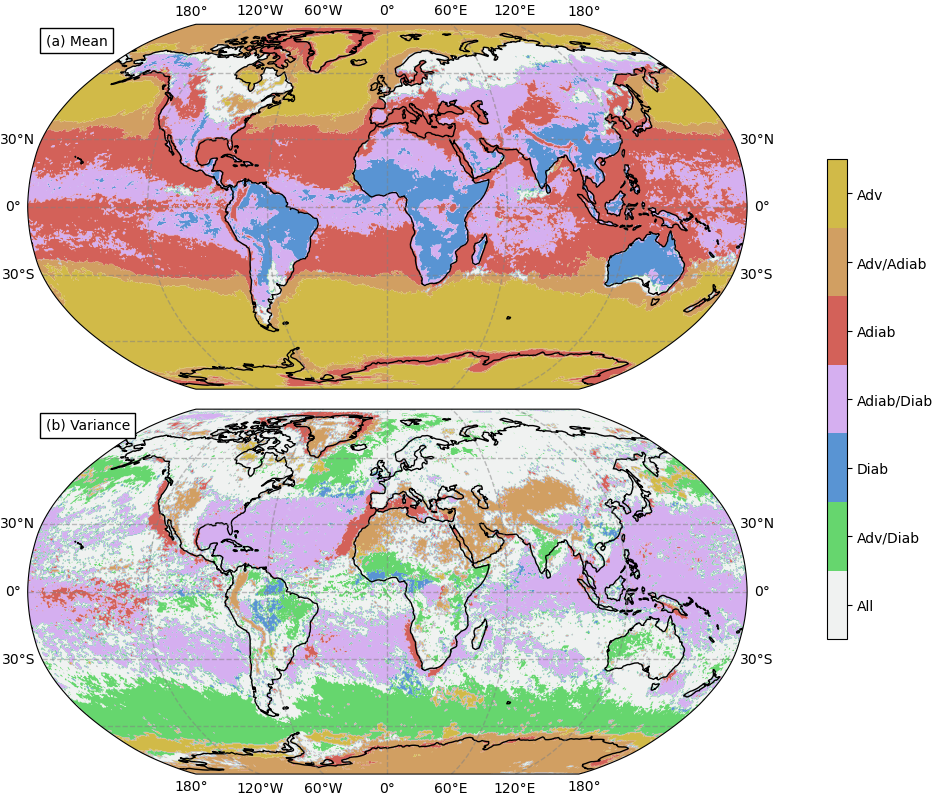
\includegraphics[width=1\linewidth]{images/dominant} \caption{(a) Reproduced from \cite{rothlisberger_quantifying_2023}. Maps at every location the most important contributor to average TX1day yearly maxima magnitude. (b) Maps at every location the most important variance term to variance of TX1day yearly maxima magnitudes. Contributor A is most important if it is 2 times larger than the second largest contributor. Contributors A and B are collectively most important if the smallest of the two is 2 times larger than the least important contributor. Else, all contributors are deemed important.}\label{fig:dominant}
\end{figure}

The coastal regions that showed peaks in TX1day \(T'\) variance are primarily dominated by adiabatic \(T'\) both in the variance and in the mean - the only contributor exhibiting perfect agreement globally. There is nonetheless a clear land-ocean contrast in the variance spatial patterns, as opposed to adiabatic dominating also over small land regions in the Mediterranean, the North-american east coast and the coast of Morocco. This indicates that the land-ocean boundaries not only strongly influence interdecadal variability of large-scale circulation patterns \citep{wake_landsea_2014}, but also local variability of hot extreme mechanisms.

Regions of high-topography mostly show adiabatic \(T'\) dominating the mean with the additional advective \(T'\) influence in the variance. This is expected given the large negative covariances between advective and adiabatic \(T'\) in these regions, suggesting that hot extreme development is modulated by mechanisms with competing processes. However, regions with advective and adiabatic \(T'\) dominance in the variance tend to cover larger areas, particularly over the Himalayas where this regions extends from the Caspian sea to Southern Mongolia, where diabatic \(T'\) is a dominating term for the mean. Katabatic winds - high-density air flows that descend higher elevation slopes due to the force of gravity, thus represented as a positive adiabatic contribution - are highly prevalent in the Himalayas due the diabatic cooling of rising air by glacial surfaces. Under climate-change, observations have shown an increase in katabatic wind activity \citep{salerno_local_2023} that then suggest the advective cooling of these flows and its dampening effect on the adiabatic parcel are more susceptible to yearly variability than the contribution from diabatic heating such as from solar radiation along the parcel trajectory and diabatic cooling due to the influence of glaciers.

Complete disagreement - i.e.~no common contributors - between the maps involve only two regions. In the Southwestern Tasman Sea, advective \(T'\) mostly dominates the mean while adiabatic and diabatic \(T'\) dominate the variance. This may have important consequences for the understanding of marine heatwave development in the Tasman sea, which are attributed to both marine and atmospheric drivers, such as the positive phase of the Asymmetric Southern Annular Mode that is associated with lower wind speeds and increased downward solar radiation \citep{gregory_atmospheric_2023}. Since this driver does not occur every year, annual changes in diabatic \(T'\) contributions may be more important than advective \(T'\) changes in distinguishing between TX1day \(T'\) magnitudes. In regions on the North-side of Asir mountain range (Arabian Peninsula), diabatic \(T'\) mean-dominance is contrasted by advective and adiabatic \(T'\) variance-dominance. In addition to the fact figure \ref{fig:vardecomp} shows strong advective - adiabatic covariance in this region, this analysis suggests that year-to-year variability of the Indian Summer Monsoon - associated with strong subsidence and strengthening of northerly wind \citep{attada_role_2019} - particularly influences hot extreme magnitude variability in the Asir mountains and in its forefront.

Although the larger influence of diabatic \(T'\) globally supports previous evidence that radiative and land surface processes dominate sub-tropical changes in summer-time near-surface temperature variability \citep{holmes_robust_2015}, this work further highlights the importance in considering all three heat-generating mechanisms. Particularly over Australia, advective processes have been understood to be dominating the observed changes in summertime near-surface temperature variability \citep{watterson_changes_2008,holmes_robust_2015}. This study agrees, but further insists that for hot extremes, both diabatic - specifically in the West - and adiabatic processes cannot be ignored.

Then the variance of TX1day \(T'\) is almost entirely dominated by more processes than its mean counterpart. The implications is that process understanding of hot extreme development, particularly over land, requires more careful examination of changes in the physical processes due to climate changes. This shows that less important mechanisms for mean characterization of TX1day events become significant when quantifying year-to-year variability.

\section{Characterizing contributor dependencies}\label{characterizing-contributor-dependencies}

The covariances discussed in \hyperref[relating-tx1day-t-variability-to-component-variability]{4.1} are useful in quantifying the importance of contributor interactions to TX1day \(T'\) variance. Since the contributors may evolve on different magnitude scales in different parts of the world, covariances may be inadequate in investigate their dependence structures. This section adjusts for the relative scales of each contributor and uses PCA to focus on characterizing the observed variability only in the contributors.

Figure \ref{fig:pcaexplainedvar} shows that there are only few regions that have over 90\% of explained variance by PC1. These are almost only over oceans and mostly in the vicinity of storm tracks - particularly between Australia and Antarctica and its coasts with over 95\% of explained variance - as well as over the tropical Pacific and in the Atlantic between Brazil and the Sahel region collocating with sea-surface temperature maxima. Additionally, the Northern Atlantic and Arctic Ocean have mostly over 80\% of variance explained by PC1.

\begin{figure}[h]
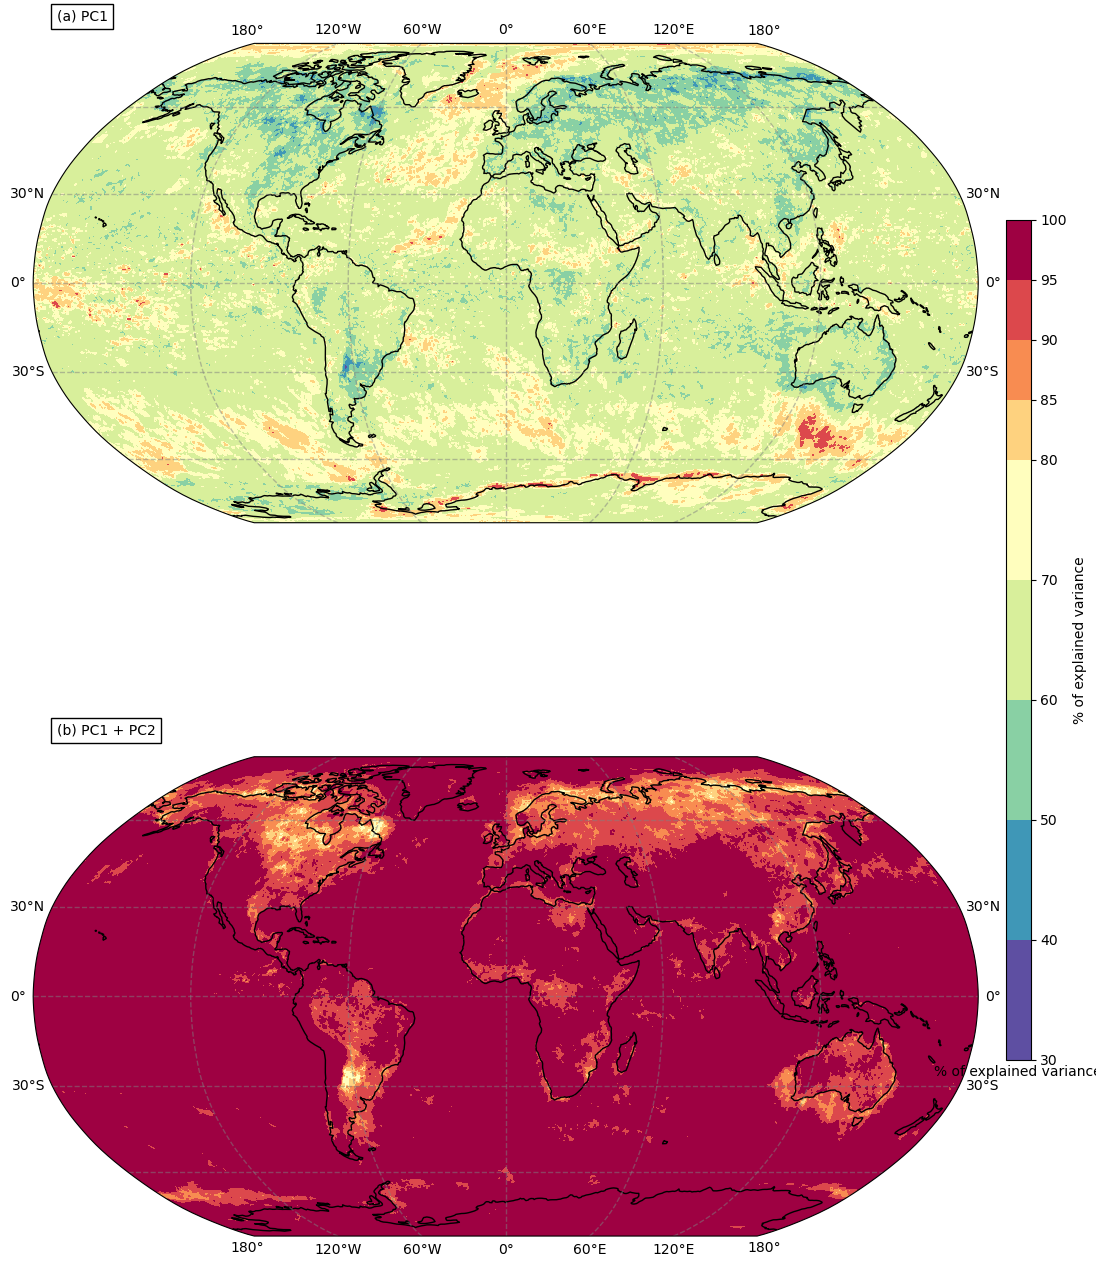
\includegraphics[width=1\linewidth]{images/pca_explainedvar3} \caption{Percentage of variance in advective, adiabatic and diabatic $T'$ that is explained by (a) PC1, (b) PC1 and PC2. The contributor directions most aligning with PC1 and PC2 - see 5.2 - for regions with at least 95\% of variance explained by PC1 and PC2 are shown in (c) and (d), respectively. Regions with less are masked in light grey.}\label{fig:pcaexplainedvar}
\end{figure}

The land regions with over 70\% of explained variance are generally limited to regions in the vicinity of high topography, but also Western and equatorial Africa and Northern Colombia. The remaining land regions have between 34 and 70\% of variance explained by PC1 - with the lowest values achieved in Northern Argentina, central Canada and Arctic Russia - and correspond to the areas requiring PC3 to explain more than 60\% of their \(T'\) variance.

The PC scores in figure \ref{fig:pcaexplainedvar} (c-d) shows that even in regions with over 95\% of the variance explained by PC1 and PC2 - although being constrained to two degrees of freedom - the PCs do not clearly align with a single or two contributors. In fact, the PC1 map supports figure \ref{fig:dominant} with very similar spatial patterns. All single-dominating regions in figure \ref{fig:dominant} are however now shown to be variable in 2 or three axes. In tropical regions, where small variances may have influenced the reliability the utilized definition of dominance, some regions with no dominating variance term now show PC1 aligning mostly with advective and either adiabtic or diabatic \(T'\). Finally, as geometrically expected, the PC2 score aligns most with the opposing contributors.

Further interpreting the PC components is difficult without considering the temporal evolution, since the PCA is applied to the final decomposition which includes aggregated contributions. Nonetheless, this analysis demonstrates that hot extreme event trajectories involve strong dependencies between the three contributors and that they may be represented using only one or two degrees of freedom. In addition, the resulting axes of variability do not align well with the original contributors, but instead mostly involve both advective and adiabatic \(T'\) over the oceans and both adiabatic and diabatic \(T'\) over land.

\section{Forecasting the last 24h of TX1day trajectories}\label{forecasting-the-last-24h-of-tx1day-trajectories}

To more specifically study the dynamics between contributors of hot extreme events, we now consider the history of parcel trajectories and model them with an LSTM-based NN architecture. Recall that the final model is trained on half of all grid-points as illustrated in figure \ref{fig:traintest} for years between 1980 to 1990. Then, figure \ref{fig:mse} shows the accuracy of this model in predicting the final 24h of advective, adiabatic and diabatic \(T'\) evolution, for the test set that consists of all grid-points for years between 1991 and 2020.

\begin{figure}[h]
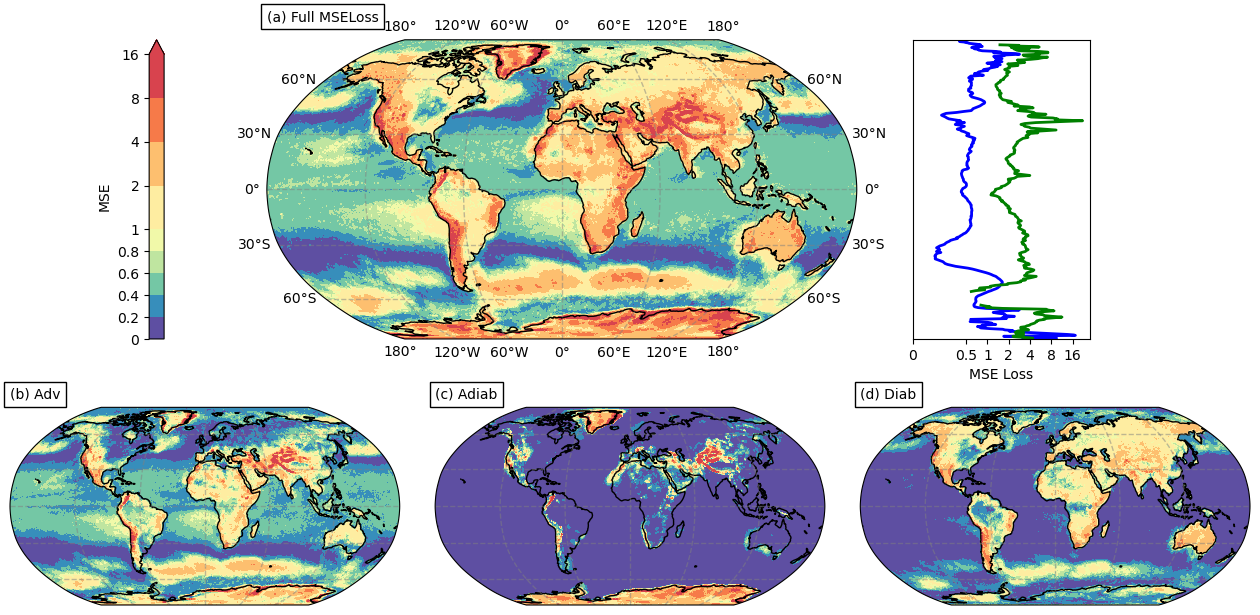
\includegraphics[width=1\linewidth]{images/mse_final} \caption{Median mean-squared-error (MSE) loss over years 1991 to 2020 for the (a) total, (b) advective, (c) adiabatic and (d) diabatic forecasts. The line graph shows oceanic and terrestrial latitudinal averages in blue and green, respectively.}\label{fig:mse}
\end{figure}

The model performs best over oceans in longitude bands between 30 and 45\(^\circ\) latitude North and South, with MSE loss lower than 0.2 for all contributors. There is a strong land-ocean contrast evident in the full forecast as well as for each contributor, with exceptions for adiabtic \(T'\) that performs very well over many land regions. The land areas that achieve low MSE loss include eastern North-America, regions east of the Andes, northern Eurasia and east China, with all three contributors being well-forecasted. The regions exhibiting the poorest performance include regions of high topography, the Arctic and Antarctic ice sheets. In addition, hotspots that were observed to have large mean and variance in section \hyperref[relating-tx1day-t-variability-to-component-variability]{5.1} such as the east coasts of Northern Africa, South and North America also have peaks in MSE loss that reach above 8\(^\circ\)C\(^2\).

Generally, the oceans are forecasted accurately, with only the advective term contributing considerable MSE loss in the tropics and both Northern and Southern storm-tracks. The two regions off the coasts of Southern Africa and South America that report 0.6 to 2\(^\circ\)C\(^2\) median MSE loss collocate approximately with SST patterns associated with with ENSO. During positive and negative phases of ENSO, SST gradients in the tropical to subtropical eastern Pacific strengthen significantly, coupled with increased wind stress \citep[for e.g.][]{chelton_observations_2001}. Poor predictability of the advective \(T'\) in this region may then be due to more diverse trends in the evolution of advective processes and their association to the ocean surface and diabatic processes. The hotspot in the Southern Atlantic may be further explained by similar SST variability associated with the South Atlantic Dipole, as well as its year-lagged teleconnection to ENSO \citep{ham_inter-basin_2021}.

Figure \ref{fig:msebase} shows the accuracy of the baseline model: constant prediction of value 27h before the event for each contributor. This reveals a number of important insights both into the data and the limited performance of the LSTM model. A low MSE loss for tropical to mid-latitudinal oceanic regions is reasonable given that they also record the lowest average \(T'\) magnitudes, with the areas that show larger mean adiabatic \(T'\) also exhibiting larger MSE loss. The baseline outperforms the LSTM model in this areas, particularly due to advective \(T'\) that is often wrongly predicted to increase by the LSTM.

\begin{figure}[h]
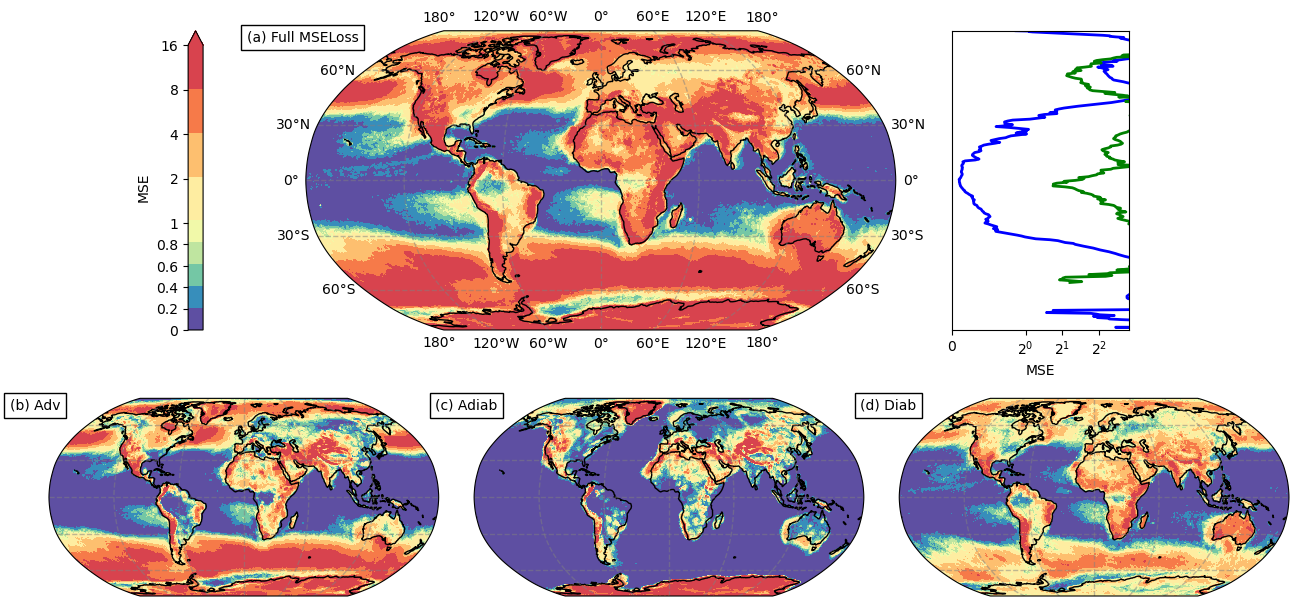
\includegraphics[width=1\linewidth]{images/mse_base} \caption{Median mean-squared-error (MSE) loss over years 1991 to 2020 for the (a) total, (b) advective, (c) adiabatic and (d) diabatic forecasts. The line graph shows oceanic and terrestrial latitudinal averages in blue and green, respectively.}\label{fig:msebase}
\end{figure}

The adiabatic term shows very small MSE loss over all oceans as well as parts of South America, eastern North American, India, Northern Eurasia and parts of Australia, suggesting that globally, little to no additional adiabatic heating occurs in the 24h preceding a TX1day event. However, previous work showed large adiabatic contributions to both mean and variance of event \(T'\). We therefore hypothesize that hot extreme events over oceans tend to evolve from parcel trajectories that descend to the surface with significant positive contributing from adiabatic \(T'\) at least 24h before the event. The final 24h period may then be dominated by diabatic \(T'\) from atmosphere interactions with the ocean surface and advective \(T'\) from prevailing circulation patterns. Exceptions occur consistently in coastal regions or in the Arctic circle, where literature supports persistent subsidence when the typical ice-sheet temperature inversion is weakened \citep{wille_extraordinary_2024}.

We further investigate the regions successfully modeled by the LSTM and not with the constant baseline model - most notably, over oceans in longitude bands between 30 and 45\(^\circ\) latitude North and South. Figure \ref{fig:msegood} shows trajectory plots a location off the coast of Japan. Previous work reports that this region is mean-dominated by advective \(T'\) and variance-dominated by advective and diabatic \(T'\), which agrees with the large increases in advective \(T'\) and large decreases in diabatic \(T'\) during the last 1 to 2 days. In 2014, the LSTM model correctly predicts this behavior even though the TX1day event trajectory is just 1 timestep longer than the forecasting window, while in 2010 and 2012 it incorrectly predicts a decreasing diabatic \(T'\) trend - this is otherwise generally correct, as seen for the remaining years. In fact, the model predicts 2\(^\circ\)C advective \(T'\) gain, approximately constant zero adiabatic \(T'\) and 0.5\(^\circ\)C diabatic \(T'\) loss when given an input of zeros. This suggests that this is the most prevalent behavior of TX1day events with short \(T'\) trajectories, since the model most likely outputs the average for timeseries when given un-informative histories as input.

Overall, the value of the LSTM model is limited as its poor ability to correctly reproduce typical dynamics means we are unable to trusts its behavior. Although outperformed over tropical oceans, it is often superior in performance against the constant baseline and this should be encouraging, indicating that in many regions, at least one of the contributor is predictable from the trajectory history. The model also generalized from the training regions to the validation regions well, as the areas of higher MSE loss do not seem to collocate with the validation locations. Then, particularly over oceans, this work suggests that forecasting future tendencies of TX1day trajectories is possible but necessitates a more complex model with more careful treatment of the inputs. We discuss potential avenues for improvement in \hyperref[limitations-and-future-work]{Chapter 6.2}.

\begin{figure}[h]
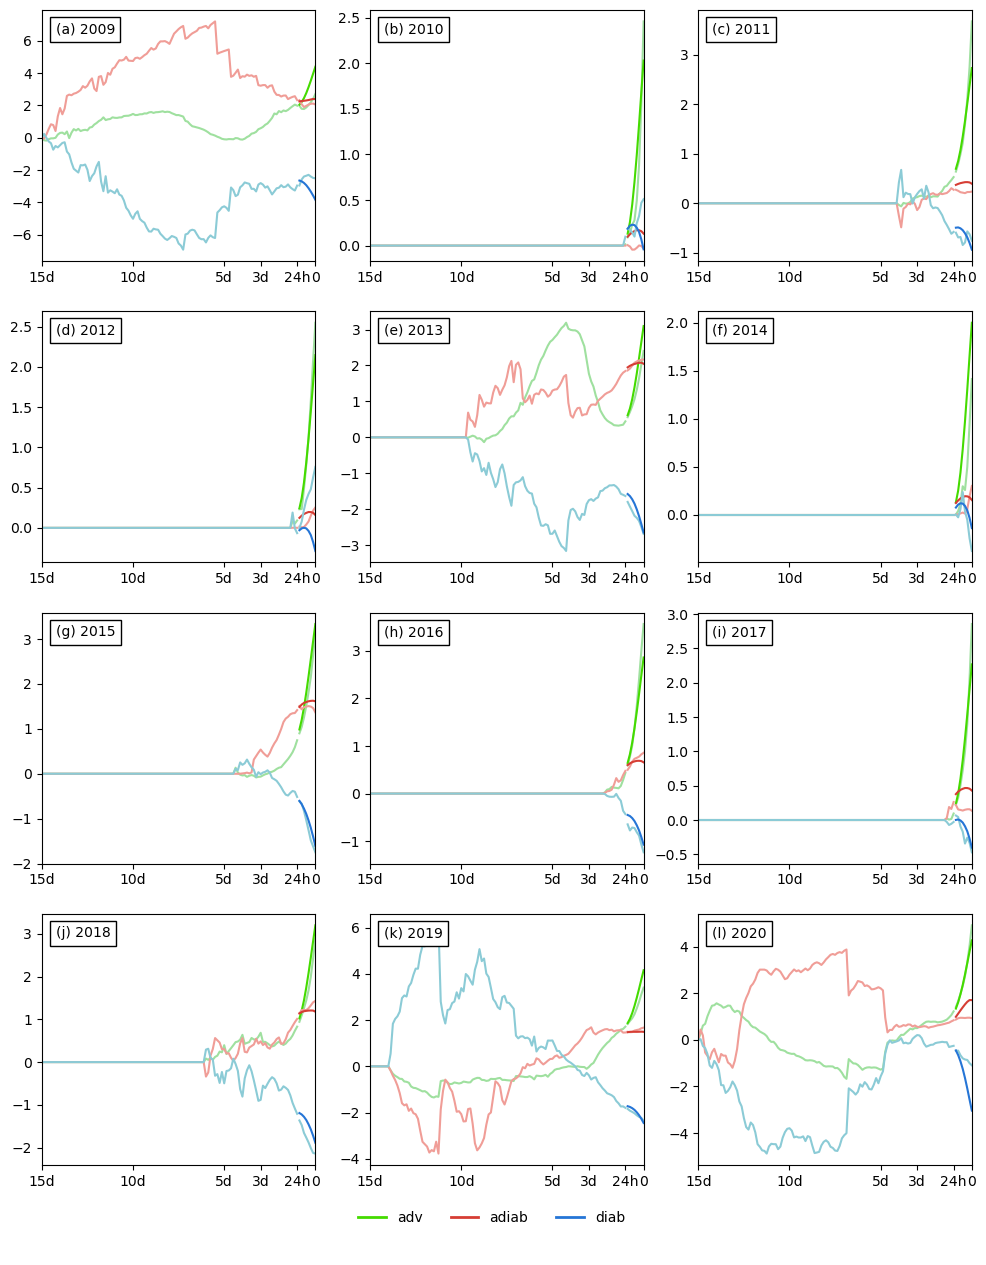
\includegraphics[width=1\linewidth]{images/msegood} \caption{Parcel trajectories and LSTM model predictions for location 38N 115E for the last 9 years of test data (2012-2020). The darker, more vibrant colors correspond to the predictions; the lighter colors correspond to the truth.}\label{fig:msegood}
\end{figure}

\chapter{Conclusion}\label{conclusion}

\section{Summary}\label{summary}

Hot extremes present a threat to human health, the economy and sensitive ecosystems. Although the variability in yearly hot extreme magnitudes has been studied and regionally linked to various physical mechanisms, a global view on these events lacks. This thesis bridges this gap by exploring the spatial variability observed in the year-to-year variability of TX1day events and link it to the year-to-year variability in the contribution from advective, adiabatic and diabatic heat-generating mechanisms. By considering the Lagrangian approach proposed by \cite{rothlisberger_quantifying_2023}, its mean-state characterizations are extended to a comprehensive second-moment analysis.

Global patterns in TX1day \(T'\) variance are found to be similar to TX1day \(T'\) magnitudes, with predominantly larger variance over land and increasing with increasing latitude. There is however more defined land-ocean contrasts, particularly on the Western coasts of continents between 25\(^\circ\) and 60\(^{\circ}\) North and 15\(^\circ\) and 60\(^\circ\) South with up to 16\(^\circ\)C\(^2\) differences in variance in just 100km. No physical process is found to dominate TX1day event variability and the processes dominating the mean exhibit again similar patterns to those in the variance. Only few local regions - including the high-variability Western coasts - have a single contributor dominating the variance and these generally agree with the mean behavior. However, dominance in the mean by a contributor does not imply dominance in the variance only by this contributor, with more complete contributions from all three processes globally. Most significantly, this analysis finds that diabatic \(T'\) variance contributions are often large, despite negative contribution in the mean. This suggests that diabatic processes through diverse land-atmosphere feedbacks and cloud-cover are important in year-to-year variability of hot extremes. This supports existing literature \citep{wehrli_identifying_2019,miralles_mega-heatwave_2014,schumacher_amplification_2019}, although finding a larger influence in the mid- to high-latitudes than \cite{wehrli_extremex_2022}.

Furthermore, the large and mostly negative covariances in \ref{fig:vardecomp} are examined through PCA, finding that most of the globe has the variability of the three contributors constrained to only one or two axes of variability. This implies that, particularly over oceans, complex mechanisms suggested by the variance decomposition and supported in the literature can be more simply characterized. In regions with variance that remains poorly explained by two axes, contributors then act more independently which may suggest the influence of a larger diversity of physical mechanisms along parcel trajectories. These areas are found in high latitudes, such as over Northern Russia and Canada, and further suggests that Arctic amplification \citep{cohen_recent_2014} may be responsible for this complexity.

The approach for the analysis of parcel trajectories was limited due to poor predictive performance in many locations. Some tendencies were learned and thus out-performed the constant baseline everywhere except in tropical regions where small temperature anomalies were exaggerated by the model. We have however shown that the patterns in advective, adiabatic and diabatic temperature anomaly generation may be predicted from their history with a relative simple model, encouraging for future work. In addition, over oceans and many land regions we observe that adiabatic heating is minimal during the final 24h, suggesting that hot extreme primarily descend to the surface earlier than a day before, thus leading to contributions from advective and diabatic processes more likely.

\section{Limitations and future work}\label{limitations-and-future-work}

Although providing novel insights into the global variability of physical processes contributing to hot extreme development, the methods proposed have several limitations. First of all, the variance decomposition only explores the year-to-year variability of the cumulative total \(T'\) contribution. A total estimate is meaningful, but it cannot easily make statements about the underlying dynamical structures. Nonetheless, together with PCA, these methods provide a unique perspective into the interactions involved in hot extreme development on a global scale.

This thesis was then largely successful in analyzing the patterns in the final cumulative trajectory data. However, many questions considering the timeseries history of TX1day event trajectories remain open. The approach to explore hot extreme dynamics with the use of DL for the modelling of final-day evolution was unsuccessful due to the model's poor performance. This work has however shown that some dependencies between contributors may be learned by even a simple model and that they are useful for forecasting next-day tendencies of each contributor. Given the large dataset considered and the diversity of timeseries behaviors, we suggest that future work should consider the following two changes. First, a revision of the data pre-processing: scaling by the median and inter-quantile range - although effective in dampening the influence of outlying values - did not transform each contributor to comparable ranges, which likely heavily biased the model to focus on limiting the loss due to the contributor with the largest scaled magnitude. Second, a more complex model may be required: this work focused on the contributors and therefore did not consider any additional trajectory information, such as geographical location and pressure level that are shown to play an important role. Given the large dataset, a sufficiently large neural network may learn to infer these features but to balance computational burden and model performance, these features may improve the ability of the model to capture changing dynamical mechanisms. In addition, increasing the number of LSTM hidden units may be required to obtain a richer feature-representation for each timeseries that can then be processed by the linear layer.

Another limitation of the model is that it was trained to predict only the last 24h in each trajectory. Although the model makes use of the full trajectory history and therefore learns important patterns in the evolution of each physical mechanism, it limits inference for the final 24h period and forces it to output an average behavior when trajectories are younger than the forecasting window. As was seen, some trajectories show little evolution in the final 24h - either for a single or multiple contributors - and therefore may learn to ignore important aspects of the hot extreme development when outputting flat forecasts. Future work may then focus on training a model on diverse input windows - i.e.~only using a set number of timesteps - to predict different sections of each trajectory. Exposing a model to different situations, rather than the complete history, would likely improve its ability to learn more meaningful dynamical patterns, thus improving predictive performance. Furthermore, prediction for various temporal regions would allow for a broader application of the model.

Finally, the model did not allow `opening the black-box' to more precisely explore the interactions between contributors and how they relate to model predictions. This requires a model that performs well on the test-data, both in terms of low MSE loss and its ability to correctly predict general trends. Given the improvements suggested above are successful in developing a better model, future work should focus on its interpretability. Explainable AI methods have received considerable attention recently and many frameworks have been extended for multivariate timeseries data. WindowSHAP \citep{nayebi_windowshap_2023} is a post-hoc method that assigns importance to windows of input multivariate timesteps. It is particularly attractive for this problem as it is computationally more efficient than other masking based methods \citep[see][for a review]{rojat_explainable_2021} and provides local explanations - for an individual samples. In the context of TX1day trajectory, it then allows the identification of important time intervals and their comparison between timeseries achieving low to high final temperature anomalies. Another approach, that further reduces computational burden, is the addition of an attention mechanism to the LSTM-model presented in this thesis. Attention-mechanisms introduce learnable parameters that are optimized to give more weight to timesteps that relate to the target, thus being more discriminating than the vanilla LSTM. They have, for example, been successful in flood forecasting applications \citep{ding_interpretable_2020}, where the attention weights can then be interpreted directly and compared between inputs.
%%%%%%%%%%%%%%%%%%%%%%%%%%%%%%%%%%%%%%%%%%%%%%%%%
%%% Bibliography                              %%%
%%%%%%%%%%%%%%%%%%%%%%%%%%%%%%%%%%%%%%%%%%%%%%%%%
\addtocontents{toc}{\vspace{.5\baselineskip}}
\cleardoublepage
\phantomsection

\bibliography{bib/bib}
\addcontentsline{toc}{chapter}{\bibname}

%% All books from our library (SfS) are already in a BiBTeX file
%% (Assbib). You can use Assbib combined with your personal BiBTeX file:
%% \bibliography{Myreferences,Assbib}. Of course, this will only work on
%% the computers at SfS, unless you copy the Assbib file
%%  --> /u/sfs/bib/Assbib.bib

%%%%%%%%%%%%%%%%%%%%%%%%%%%%%%%%%%%%%%%%%%%%%%%%%
%%% Appendices (if needed)                    %%%
%%%%%%%%%%%%%%%%%%%%%%%%%%%%%%%%%%%%%%%%%%%%%%%%%
\addtocontents{toc}{\vspace{.5\baselineskip}}
\appendix
\chapter{Supplementary material on timeseries data}

\section{Further examples of trajectory data}

Find below the trajectory timeseries visualisation plots - as figure 3.2 - for the locations in figure 3.1. Each figure contains plots (a-d) of TX1day T’ decompositions for years 1980 to 2020. The x-axis is logarithmic to better represent the recent history. The trajectory yielding the largest final $T'$ among all years is colored red, the time-mean of all trajectories in black and the inter-quantile range is highlighted in light blue. Plot (e) shows the (auto-)correlation between the final $T'$ and the $T'$ at different lags for the event and each contributor. Plot (f) shows the (cross-)correlation between the final event $T'$ and the $T'$ at different lags for each contributor. They are computed for all samples that have genesis time earlier than the considered time-lag.

\begin{figure}[h]
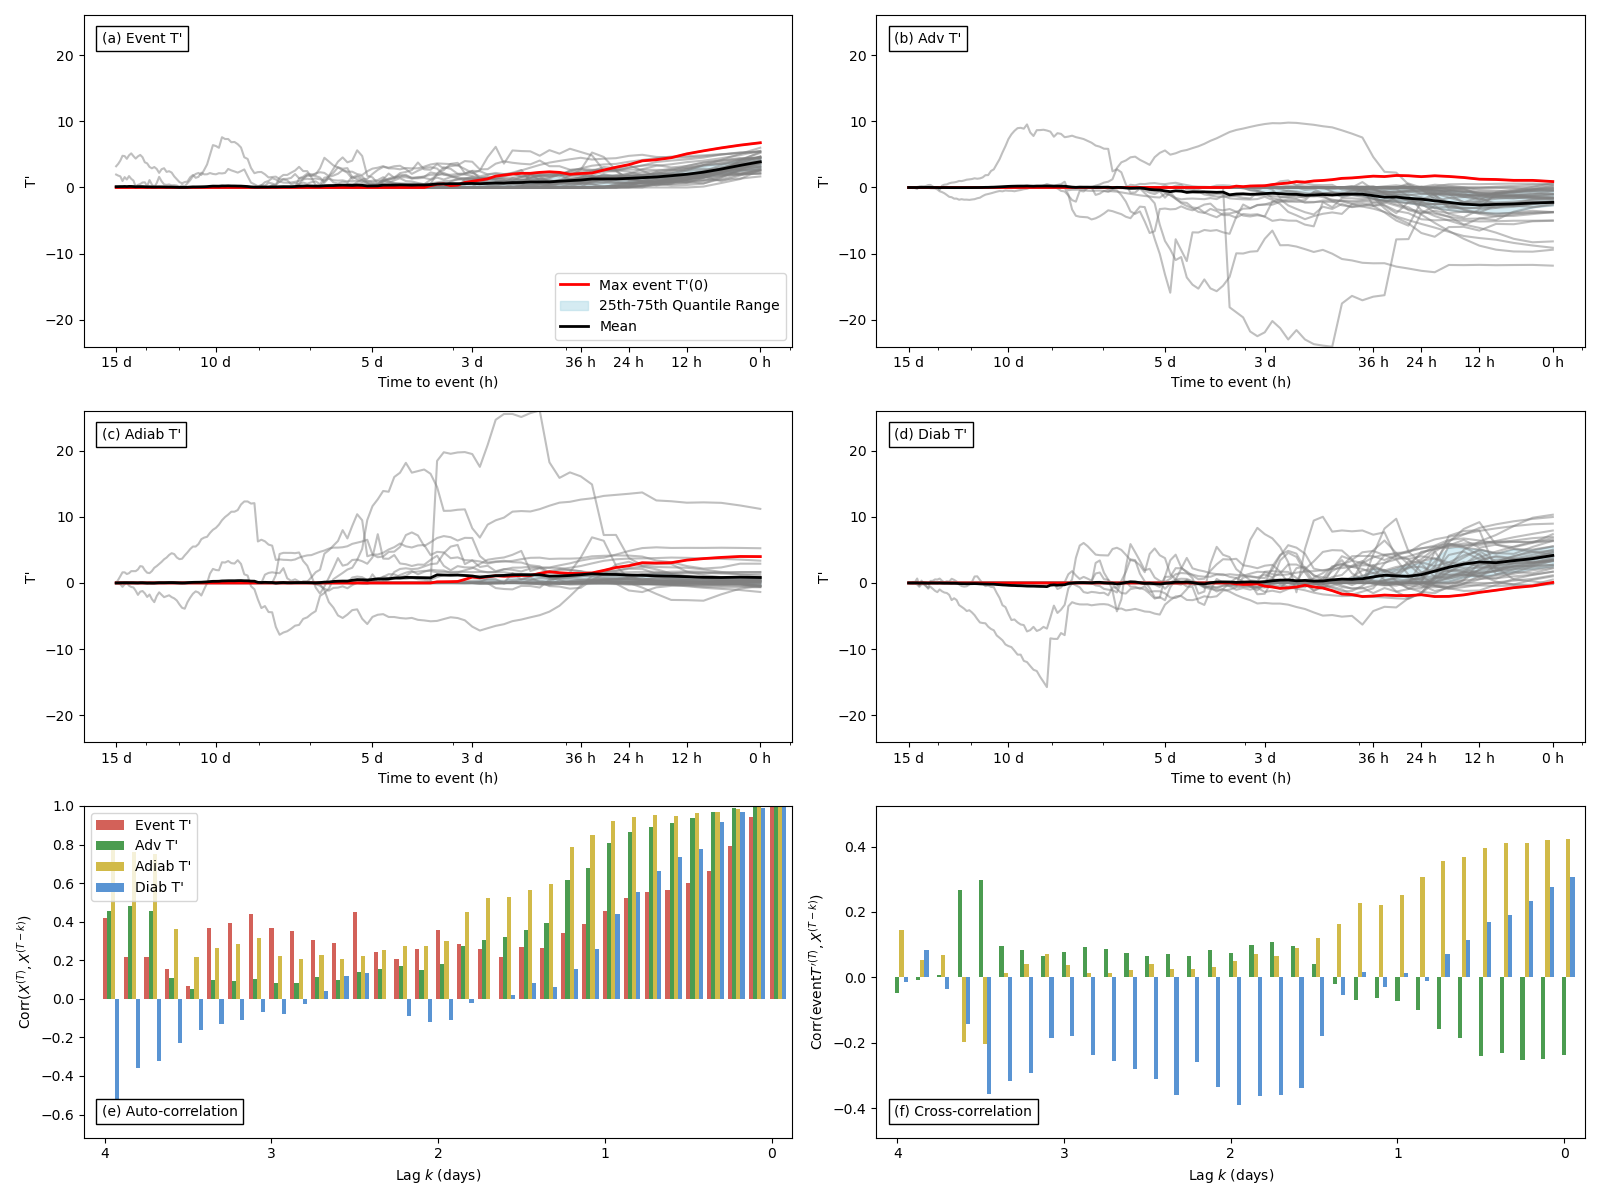
\includegraphics[width=\textwidth]{images/sup1.png}
\caption{Gridpoint 28.5N 77E located in the vicinity of New Delhi (India)}
\end{figure}

\begin{figure}[h]
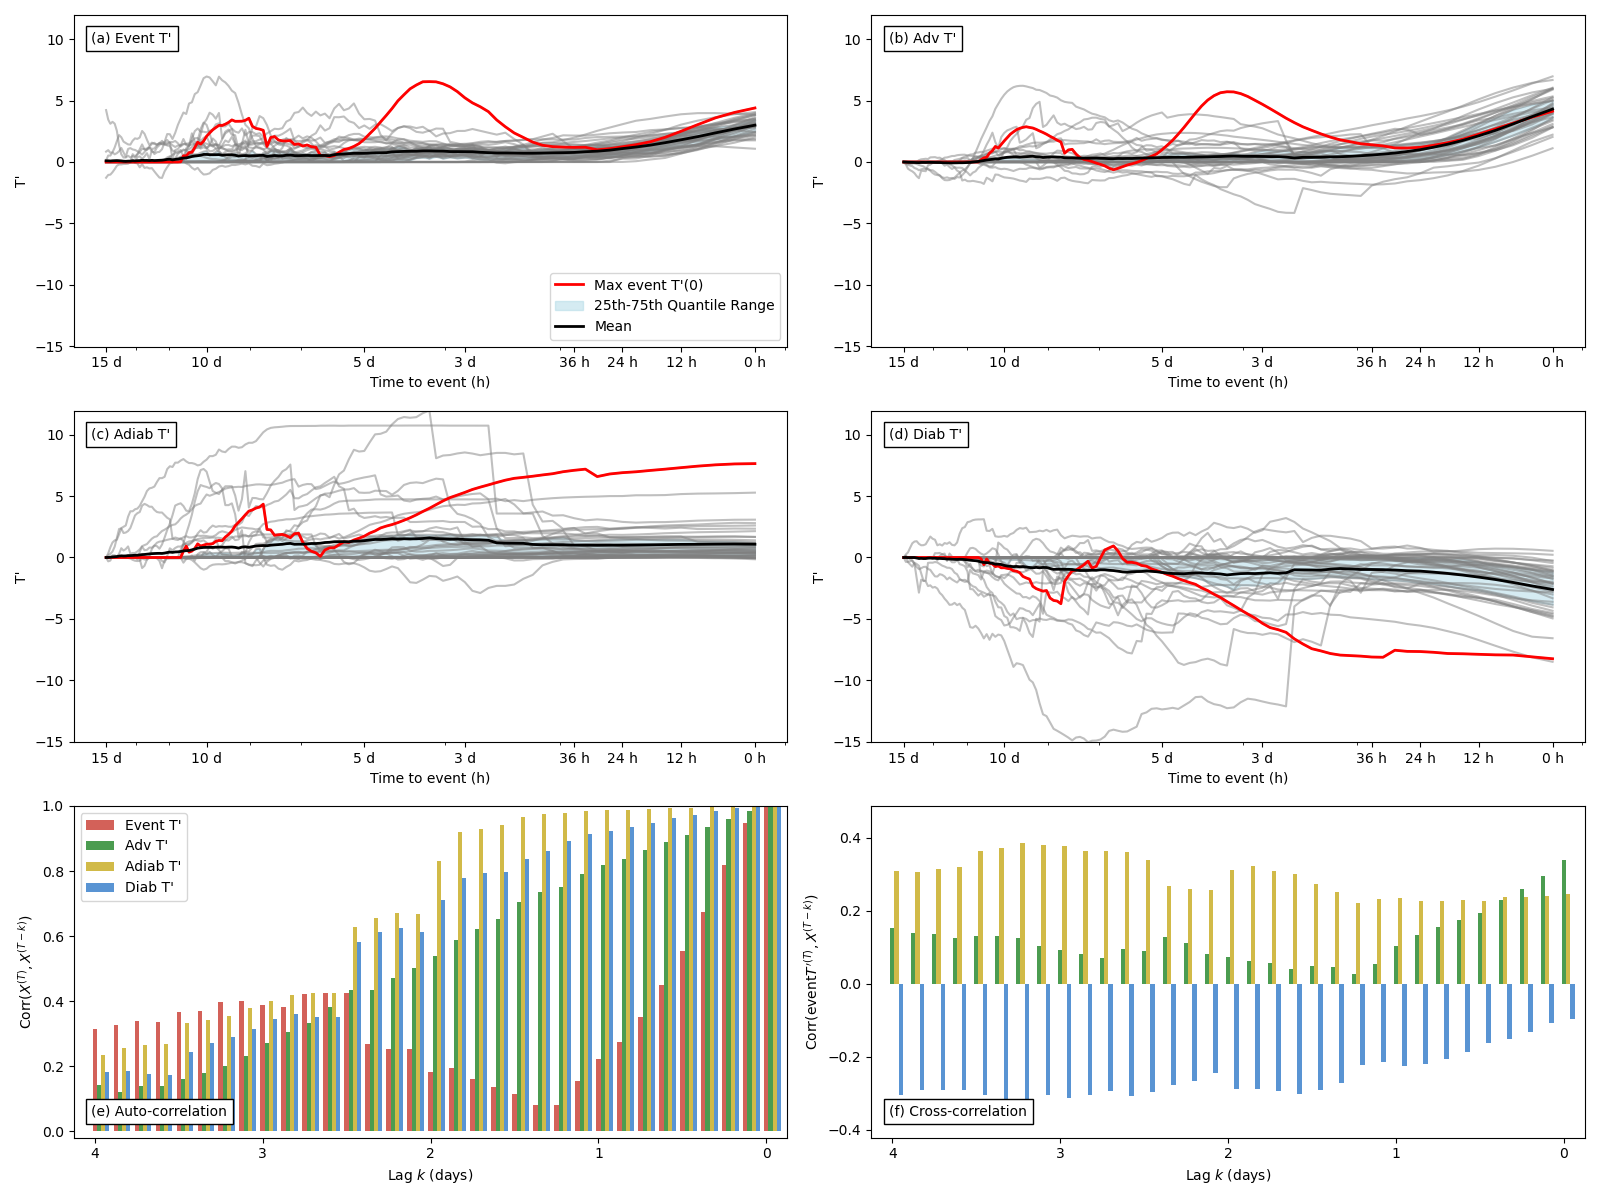
\includegraphics[width=\textwidth]{images/sup2.png}
\caption{Gridpoint 45N 30W located in the middle of the Atlantic ocean.}
\end{figure}

\begin{figure}[h]
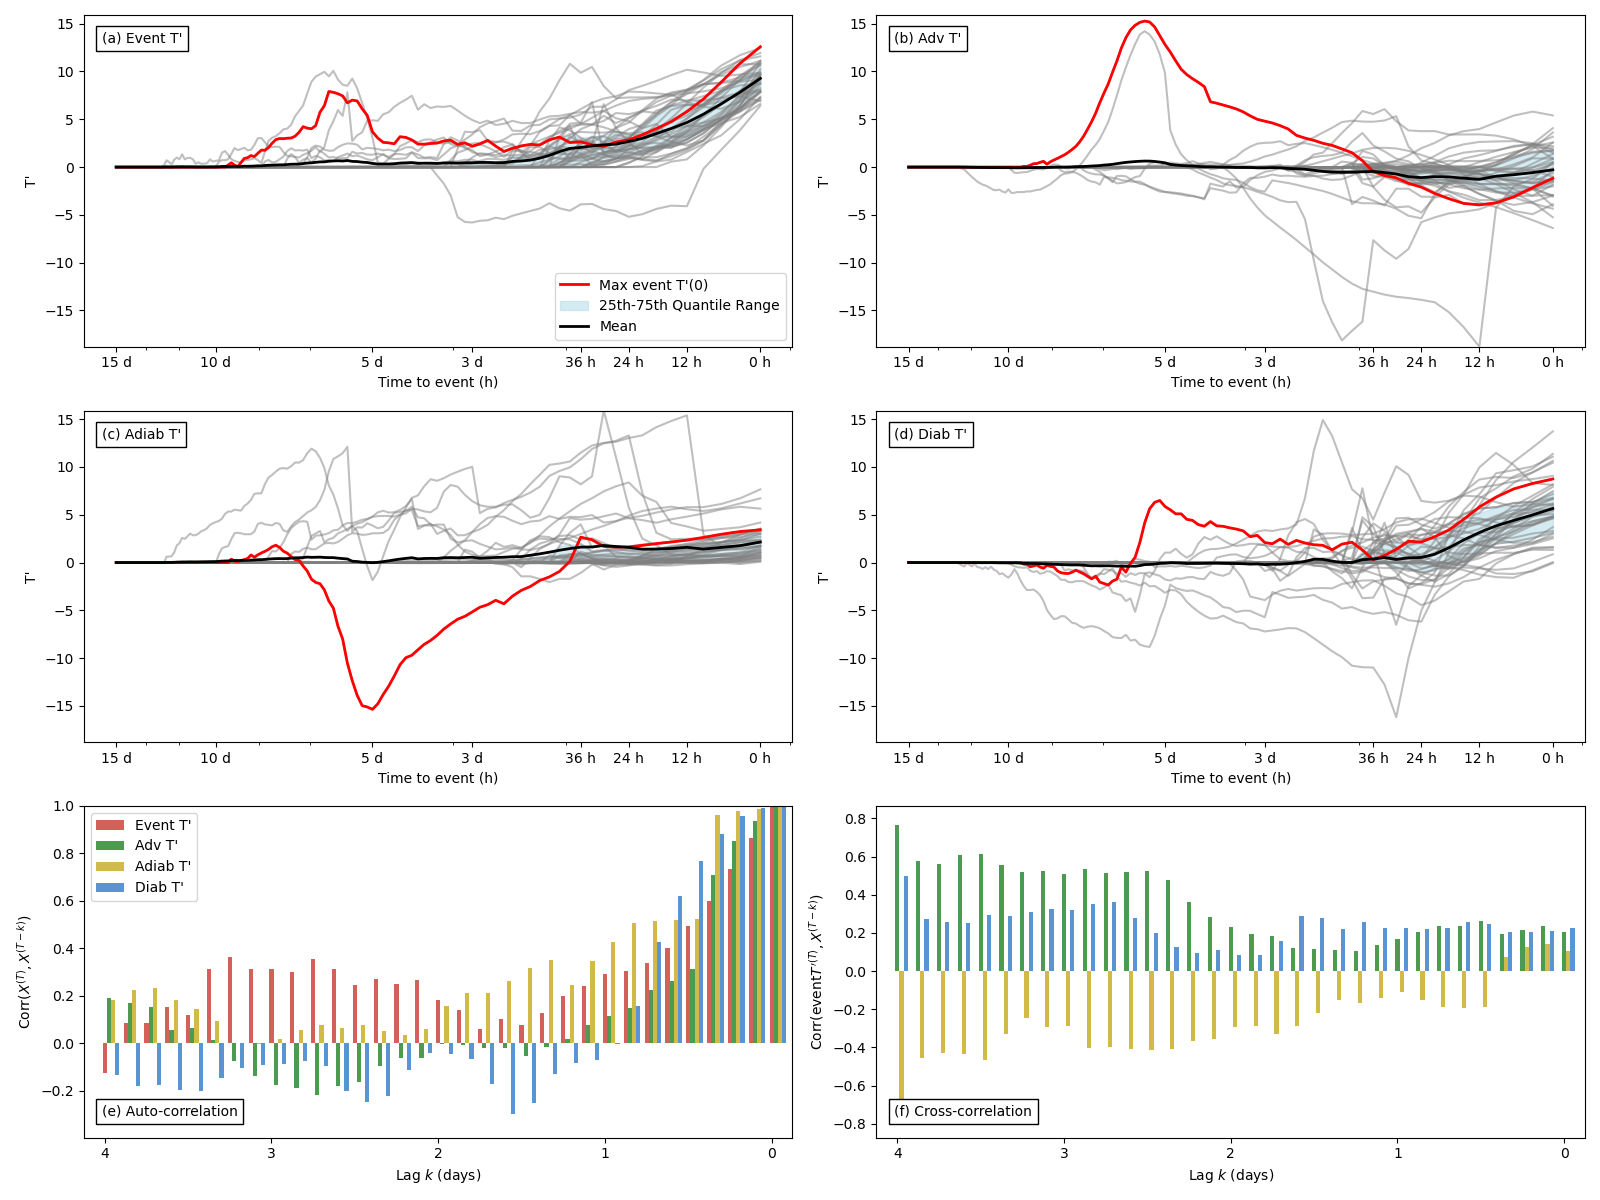
\includegraphics[width=\textwidth]{images/sup3.png}
\caption{Gridpoint 32S 116E located in the vicinity of Perth (Australia).}
\end{figure}

%%% Local Variables: 
%%% mode: latex
%%% TeX-master: "MasterThesisSfS"
%%% End: 

\section{Differenced timeseries data}

\begin{figure}[h]
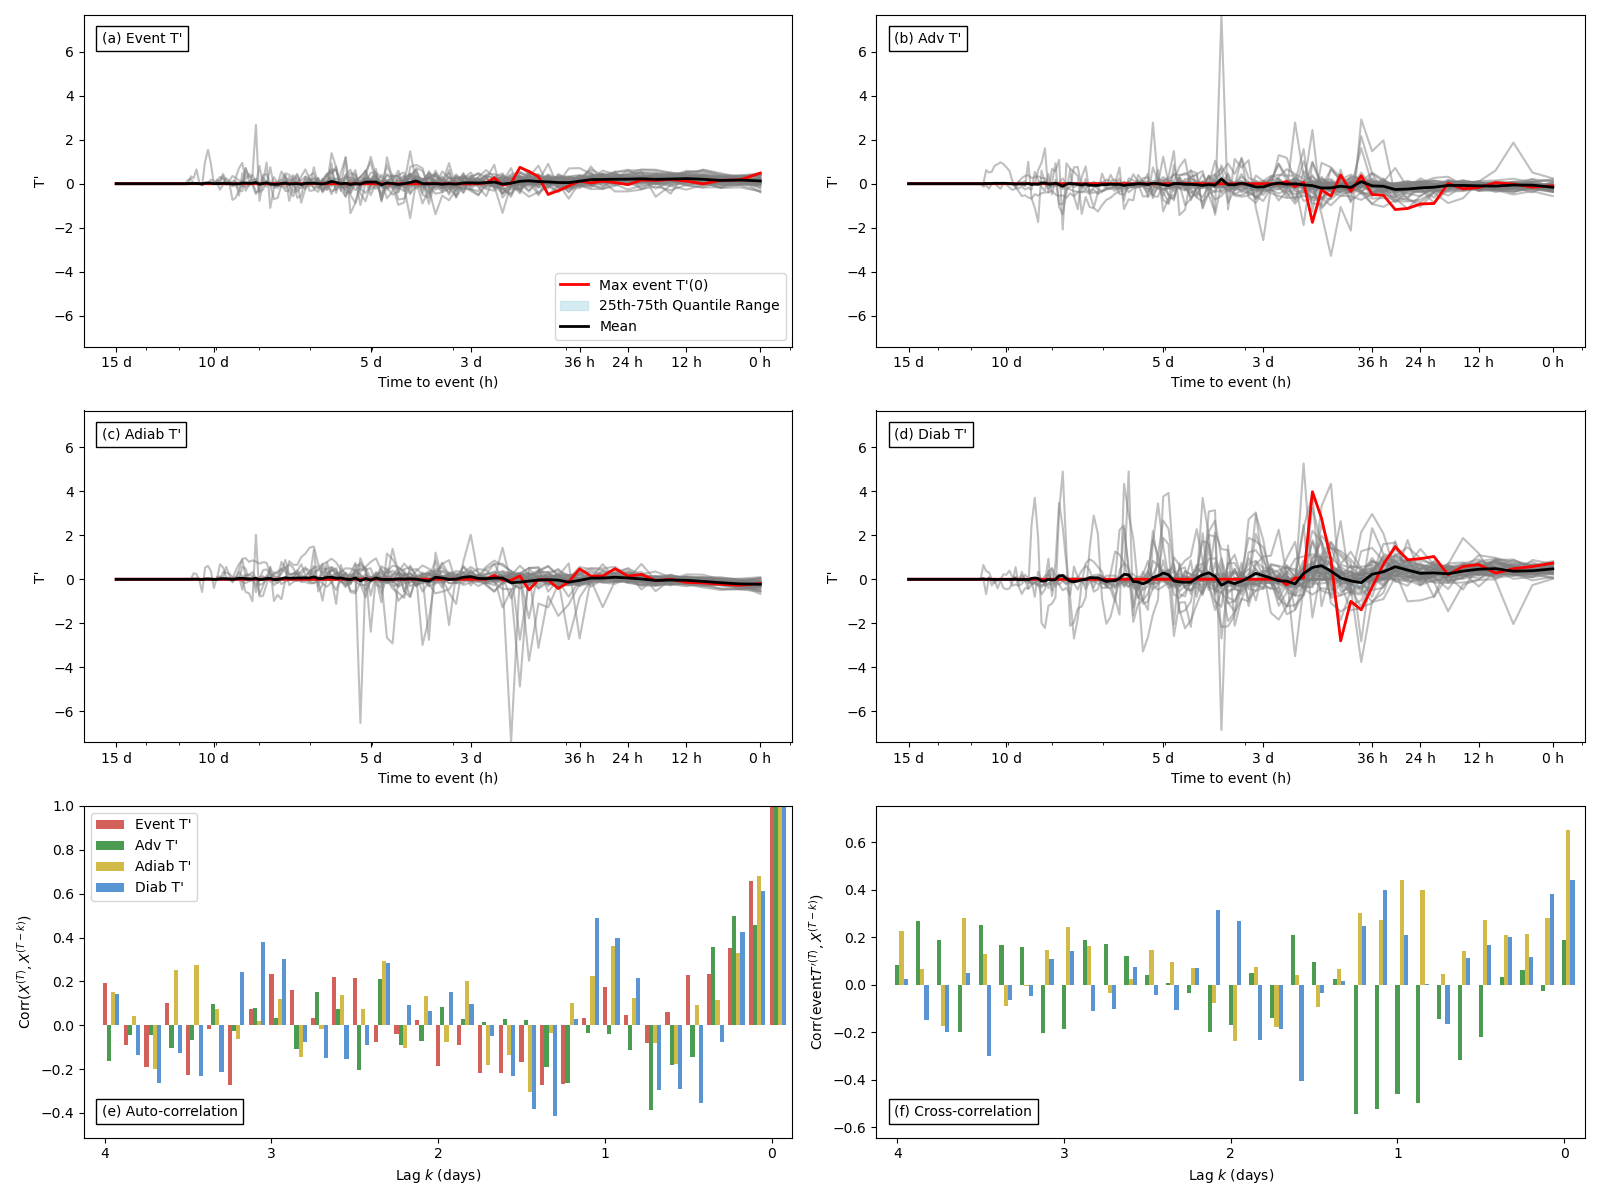
\includegraphics[width=\textwidth]{images/sup_diff.png}
\caption{Differenced timeseries visualisation plots for location 16S 48W and years between 1980 and 2020. Explanations of each graph are the same as for Appendix A.1.}
\end{figure}

%%% Local Variables: 
%%% mode: latex
%%% TeX-master: "MasterThesisSfS"
%%% End: 
\chapter{Further background on variance}

Variance is a measure of dispersion - or spread - of a distribution and is defined as the expected squared deviation from the mean. Given random variable $X \sim \mathcal{F}$, the variance of $X$ is given by $\mathbb{V}[X] = \mathbb{E}\left[ (X-\mathbb{E}[X])^2 \right]$. Conversely to the expectation, variance is a non-linear operator. Given two random variables $X \sim \mathcal{F}_X$ and $Y \sim \mathcal{F}_Y$: 
\begin{equation}
\begin{aligned}
\mathbb{V}[X+Y] & = \mathbb{E}\left[ (X+Y - \mathbb{E}[X+Y])^2\right] \\
& = \mathbb{E} \left[ (X - \mathbb{E}[X])^2\right] + \mathbb{E} \left[ (Y - \mathbb{E}[Y])^2\right] + 2 \, \mathbb{E}\left[ (X - \mathbb{E}[X])(Y-\mathbb{E}[Y]) \right] \\
& = \mathbb{V}[X] + \mathbb{V}[Y] + 2 \, \mathbb{C}\text{ov}[X,Y]
\end{aligned}
%(\#eq:vardef)
\end{equation}

by linearity of the expectation. The last term is called the covariance between $X$ and $Y$ and is a measure of linear association between two random variables. Trivially, the covariance between $X$ and $X$ is the variance of $X$.

These quantities serve as the basis for most statistical models. Normalizing covariance by the square-root of the variance of $X$ and $Y$ yields the Pearson correlation coefficient $\rho_{X,Y}$ that is often preferred as a summary measure of linear association since it can be compared between random variables with different scales. In regression, other common measure of association between the response $Y$ and one or more predictors $X_{1:k}$ includes the coefficient of determination $R^2$ measuring the proportion of the variance of $Y$ that is predicted by $X_{1:k}$.

In practice, one often assumed that observed data samples $\{(x_{1},y_{1}),...,(x_n,y_n)\}$ are independent draws from some joint distribution. Then, assuming that the mean and covariance of the distribution are finite, the following provide the sample estimates of the variance of the marginal distributions $\hat{\mathbb{V}}$ and the covariance of the joint distribution $\hat{\mathbb{C}\text{ov}}$:

\begin{equation}
\begin{aligned}
\hat{\mathbb{V}}[\{x_{1:n}\}] &= \frac{1}{n-1} \sum_{i=1}^n \left( x_i - \bar{x} \right)^2 \\
\hat{\mathbb{C}\text{ov}}[\{x_{1:n}\},\{y_{1:n}\}] &= \frac{1}{n-1} \sum_{i=1}^n ( x_i - \bar{x})(y_i - \bar{y})
\end{aligned}
%(\#eq:samplevar)
\end{equation}

where $\bar{x} = \frac{1}{n} \sum_{i=1}^{n} x_i$ is the sample mean of $X$. Note the normalizing factor $n-1$ that ensures the estimate is unbiased - in repeated sampling, the average estimates equal the true quantity. 


%%% Local Variables: 
%%% mode: latex
%%% TeX-master: "MasterThesisSfS"
%%% End: 
\chapter{Grid-search results}

Although the minimal loss was achieved by the model with no L2-regularization, it is expected that training on more than 30 times the number of samples will require some regularization. In addition, the difference in performance between models with 88 and 64 is small and thus prefer a less complex model. The final model then has parameters 64 hidden units and L2-regularization parameter $1e-06$. 

\begin{figure}[h]
\centering
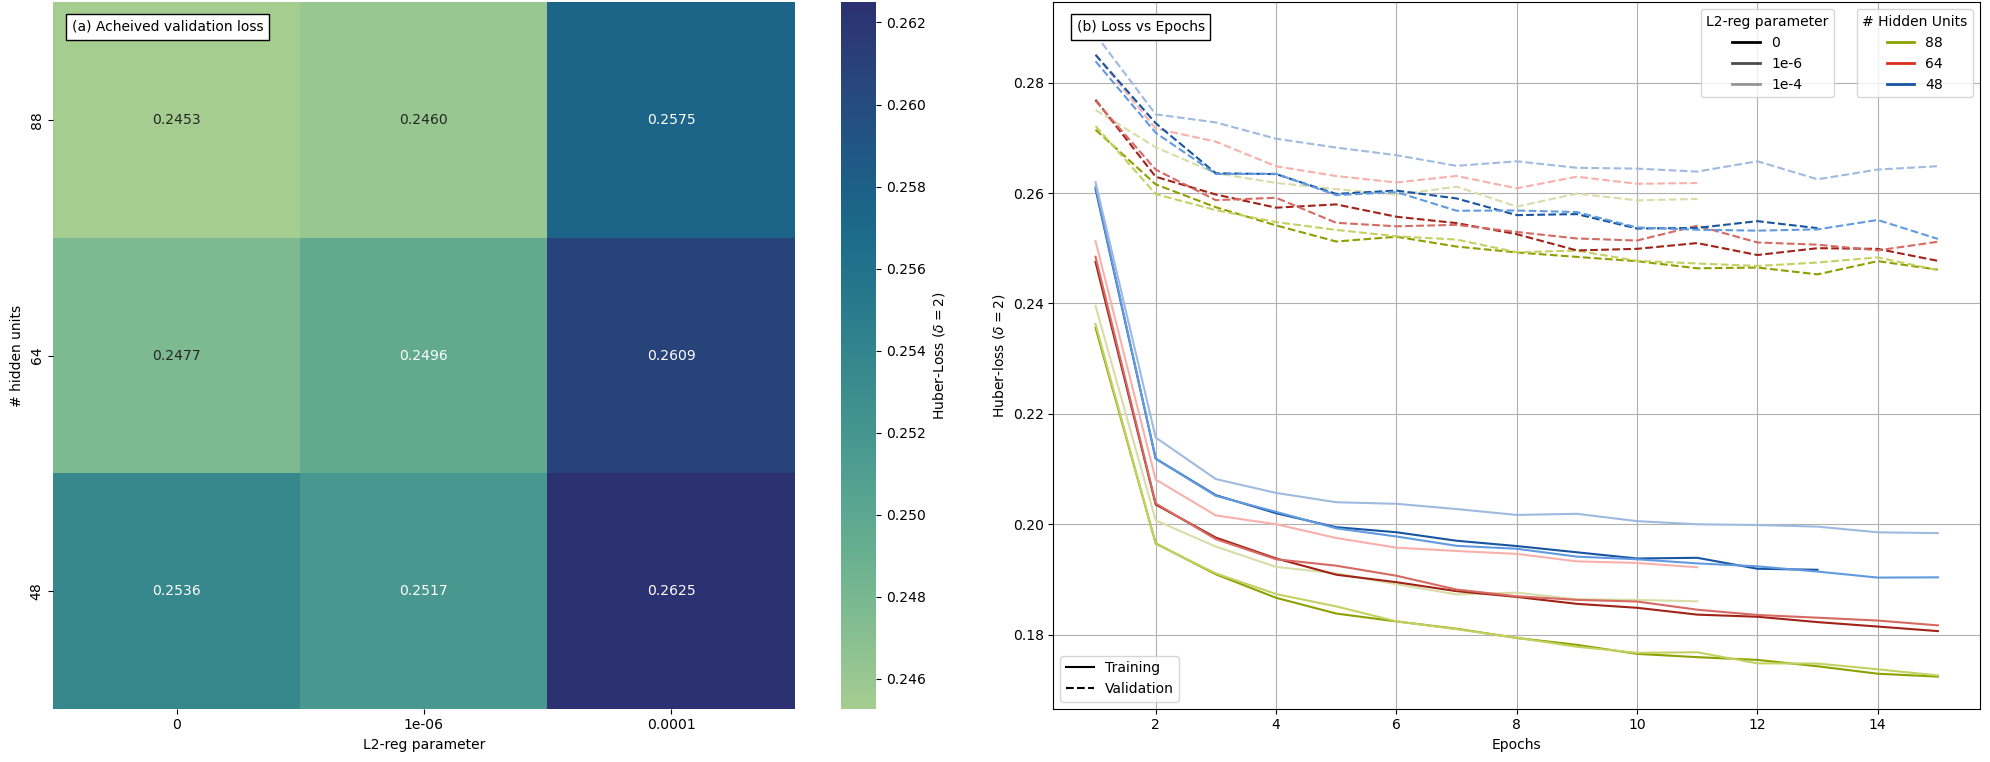
\includegraphics[width=\textwidth]{images/param_val.png}
\caption{Parameter validation results showing (a) the minimally achieved loss for each model instance and (b) the training and validation loss curves over epochs for each model instance.}
\end{figure}


%%% Local Variables: 
%%% mode: latex
%%% TeX-master: "MasterThesisSfS"
%%% End: 


%%%%%%%%%%%%%%%%%%%%%%%%%%%%%%%%%%%%%%%%%%%%%%%%%%
%%% Declaration of originality (Do not remove!)%%%
%%%%%%%%%%%%%%%%%%%%%%%%%%%%%%%%%%%%%%%%%%%%%%%%%%
%% Instructions:
%% -------------
%% fill in the empty document confirmation-originality.pdf electronically
%% print it out and sign it
%% scan it in again and save the scan in this directory with name
%% confirmation-originality-scan.pdf
%%
%% General info on plagiarism:
%% https://www.ethz.ch/students/en/studies/performance-assessments/plagiarism.html
\cleardoublepage

\includepdf[pages={-}, frame=true,scale=1]{pdf/confirmation-originality.pdf}
\end{document}
